% Version 3.3 June 2016
%
% % % % % % % % % % % % % % % % % % % % % %
%
% -- IMPORTANT NOTE
%
% This template contains comments intended 
% to minimize problems and delays during our production 
% process. Please follow the template instructions
% whenever possible.
%
% % % % % % % % % % % % % % % % % % % % % % % 
%
% Once your paper is accepted for publication, 
% PLEASE REMOVE ALL TRACKED CHANGES in this file 
% and leave only the final text of your manuscript. 
% PLOS recommends the use of latexdiff to track changes during review, as this will help to maintain a clean tex file.
% Visit https://www.ctan.org/pkg/latexdiff?lang=en for info or contact us at latex@plos.org.
%
%
% There are no restrictions on package use within the LaTeX files except that 
% no packages listed in the template may be deleted.
%
% Please do not include colors or graphics in the text.
%
% The manuscript LaTeX source should be contained within a single file (do not use \input, \externaldocument, or similar commands).
%
% % % % % % % % % % % % % % % % % % % % % % %
%
% -- FIGURES AND TABLES
%
% Please include tables/figure captions directly after the paragraph where they are first cited in the text.
%
% DO NOT INCLUDE GRAPHICS IN YOUR MANUSCRIPT
% - Figures should be uploaded separately from your manuscript file. 
% - Figures generated using LaTeX should be extracted and removed from the PDF before submission. 
% - Figures containing multiple panels/subfigures must be combined into one image file before submission.
% For figure citations, please use "Fig" instead of "Figure".
% See http://journals.plos.org/plosone/s/figures for PLOS figure guidelines.
%
% Tables should be cell-based and may not contain:
% - spacing/line breaks within cells to alter layout or alignment
% - do not nest tabular environments (no tabular environments within tabular environments)
% - no graphics or colored text (cell background color/shading OK)
% See http://journals.plos.org/plosone/s/tables for table guidelines.
%
% For tables that exceed the width of the text column, use the adjustwidth environment as illustrated in the example table in text below.
%
% % % % % % % % % % % % % % % % % % % % % % % %
%
% -- EQUATIONS, MATH SYMBOLS, SUBSCRIPTS, AND SUPERSCRIPTS
%
% IMPORTANT
% Below are a few tips to help format your equations and other special characters according to our specifications. For more tips to help reduce the possibility of formatting errors during conversion, please see our LaTeX guidelines at http://journals.plos.org/plosone/s/latex
%
% For inline equations, please be sure to include all portions of an equation in the math environment.  For example, x$^2$ is incorrect; this should be formatted as $x^2$ (or $\mathrm{x}^2$ if the romanized font is desired).
%
% Do not include text that is not math in the math environment. For example, CO2 should be written as CO\textsubscript{2} instead of CO$_2$.
%
% Please add line breaks to long display equations when possible in order to fit size of the column. 
%
% For inline equations, please do not include punctuation (commas, etc) within the math environment unless this is part of the equation.
%
% When adding superscript or subscripts outside of brackets/braces, please group using {}.  For example, change "[U(D,E,\gamma)]^2" to "{[U(D,E,\gamma)]}^2". 
%
% Do not use \cal for caligraphic font.  Instead, use \mathcal{}
%
% % % % % % % % % % % % % % % % % % % % % % % % 
%
% Please contact latex@plos.org with any questions.
%
% % % % % % % % % % % % % % % % % % % % % % % %

\documentclass[10pt,letterpaper]{article}
\usepackage[top=0.85in,left=2.75in,footskip=0.75in]{geometry}

% amsmath and amssymb packages, useful for mathematical formulas and symbols
\usepackage{amsmath,amssymb}

% Use adjustwidth environment to exceed column width (see example table in text)
\usepackage{changepage}

% Use Unicode characters when possible
\usepackage[utf8x]{inputenc}

% textcomp package and marvosym package for additional characters
\usepackage{textcomp,marvosym}

% cite package, to clean up citations in the main text. Do not remove.
\usepackage{cite}

% Use nameref to cite supporting information files (see Supporting Information section for more info)
\usepackage{nameref,hyperref}

% line numbers
\usepackage[right]{lineno}

% ligatures disabled
\usepackage{microtype}
\DisableLigatures[f]{encoding = *, family = * }

% color can be used to apply background shading to table cells only
\usepackage[table]{xcolor}

% array package and thick rules for tables
\usepackage{array}

% create "+" rule type for thick vertical lines
\newcolumntype{+}{!{\vrule width 2pt}}

% create \thickcline for thick horizontal lines of variable length
\newlength\savedwidth
\newcommand\thickcline[1]{%
  \noalign{\global\savedwidth\arrayrulewidth\global\arrayrulewidth 2pt}%
  \cline{#1}%
  \noalign{\vskip\arrayrulewidth}%
  \noalign{\global\arrayrulewidth\savedwidth}%
}

% \thickhline command for thick horizontal lines that span the table
\newcommand\thickhline{\noalign{\global\savedwidth\arrayrulewidth\global\arrayrulewidth 2pt}%
\hline
\noalign{\global\arrayrulewidth\savedwidth}}

\usepackage{soul}
% Remove comment for double spacing
\usepackage{setspace} 
\doublespacing

% Text layout
\raggedright
\setlength{\parindent}{0.5cm}
\textwidth 5.25in 
\textheight 8.75in

% Bold the 'Figure #' in the caption and separate it from the title/caption with a period
% Captions will be left justified
\usepackage[aboveskip=1pt,labelfont=bf,labelsep=period,justification=raggedright,singlelinecheck=off]{caption}
\renewcommand{\figurename}{Fig}

% Use the PLoS provided BiBTeX style
\bibliographystyle{plos2015}

% Remove brackets from numbering in List of References
\makeatletter
\renewcommand{\@biblabel}[1]{\quad#1.}
\makeatother

% Leave date blank
\date{}

% Header and Footer with logo
\usepackage{lastpage,fancyhdr,graphicx}
\usepackage{epstopdf}
\pagestyle{myheadings}
\pagestyle{fancy}
\fancyhf{}
\setlength{\headheight}{27.023pt}
\lhead{
\includegraphics[width=2.0in]{PLOS-submission.pdf}}
\rfoot{\thepage/\pageref{LastPage}}
\renewcommand{\footrule}{\hrule height 2pt \vspace{2mm}}
\fancyheadoffset[L]{2.25in}
\fancyfootoffset[L]{2.25in}
\lfoot{\sf PLOS}

%% Include all macros below
% Self-imported packages for table
\usepackage{multirow}
\usepackage{hhline}

\newcommand{\lorem}{{\bf LOREM}}
\newcommand{\ipsum}{{\bf IPSUM}}

\newcommand{\R}{\ensuremath{\mathbb{R}}}
\newcommand{\dist}{\ensuremath{\text{dist}}}
\newtheorem{definition}{Definition}

%% END MACROS SECTION


\begin{document}
\vspace*{0.2in}

% Title must be 250 characters or less.
\begin{flushleft}
{\Large
\textbf\newline{A Comparative Analysis of Trajectory Similarity Measures: Recommendations for Selection and Use} % Please use "title case" (capitalize all terms in the title except conjunctions, prepositions, and articles).
}
\newline
% Insert author names, affiliations and corresponding author email (do not include titles, positions, or degrees).
\\
Alan Both\textsuperscript{1}
Kevin Buchin\textsuperscript{2},
Matt Duckham\textsuperscript{1},
Patrick Laube\textsuperscript{3},
Dongliang Peng\textsuperscript{4},
Ross S. Purves\textsuperscript{5},
Stef Sijben\textsuperscript{2},
Rodrigo I. Silveira\textsuperscript{6},
Yaguang Tao\textsuperscript{1},
Kevin Toohey\textsuperscript{7}
\\
\bf{1} School of Science, RMIT University, Melbourne, Victoria, Australia
\\
\bf{2} Department of Mathematics and Computer Science, TU Eindhoven, Netherlands
\\
\bf{3} Institute of Natural Resource Sciences, Z\"urich University of Applied Sciences, W\"adenswil, Switzerland
\\
\bf{4} Institute of Computer Science, University of W\"urzburg, W\"urzburg, Germany
\\
\bf{5} Department of Geography, University of Zurich, Zurich, Switzerland
\\
\bf{6} Departament de Matemàtiques, Universitat Politècnica de Catalunya, Barcelona, Spain
\\
\bf{7} University of Melbourne, Melbourne, Australia
\\

\bigskip

% Insert additional author notes using the symbols described below. Insert symbol callouts after author names as necessary.
% 
% Remove or comment out the author notes below if they aren't used.
%
% Primary Equal Contribution Note
Authors Buchin, Duckham, Laube, Peng, Purves, Sijben, Silveira contributed equally to the design of this work.

Authors Both, Buchin, Tao, Toohey, Sijben contributed equally to the implementation of this work.

Authors Both, Buchin, Duckham, Laube, Purves, Sijben, Silveira contributed equally to the writing of this paper. 

% Use the asterisk to denote corresponding authorship and provide email address in note below.
* alan.both@rmit.edu.au

\end{flushleft}
% Please keep the abstract below 300 words
\section*{Abstract}

This paper describes an exploration and comparison of trajectory similarity measures, in order to make practical and generalizable recommendations for researchers seeking to use such measures. Specifically, we compare: dynamic time warping (DTW), edit distance (EDR), longest common subsequence (LCSS), discrete Fréchet distance (DFD), and Fréchet distance (FD). To clarify differences between measures, we calculate similarities for trajectories with contrasting properties: data about bus movements around a transportation network; and the movements of wading birds in a coastal environment. To examine the chosen similarity measures, four experiments were devised: creating a measurement baseline by comparing similarity measures to a single trajectory after applying various transformations; exploring the behavior of similarity measures on network constrained bus trajectories, grouping trajectories based on spatial and on temporal similarity; assessing similarity with respect to existing behavioral labels (flight and foraging of oystercatchers); and comparing bird and bus activity to examine whether they are distinguishable based solely on their movement patterns. Our results and conclusions provide practical advice and recommendations for selecting and using trajectory similarity measures across three complementary perspectives: conceptual, theoretical, and empirical. 

% Throughout all experiments, it was found that DTW, DFD, and FD perform well, while LCSS and EDR perform poorly. Additionally, spatial factors tend to be far more influential than temporal factors in determining similarity, with the second experiment indicating that spatially distant bus trajectories exhibit very little similarity, and temporal differences exhibiting no significant influence. It was also found that trajectories tend to be more diverse when they are clustered based on a more general pattern, with some patterns proving harder to extract. The diversity of trajectories for flight activity as opposed to foraging activity shown by the third experiment is a clear example of this. 

\section{Introduction}
Trajectories---recording the evolving position of objects in geographic space and time---are fundamental building blocks of computational movement analysis~\cite{DBLP:series/sbcs/Laube14}. Trajectories have become ubiquitous in a wide range of domains. These domains range across spatial and temporal scales, from analysis at the scale of micro-organisms in laboratory settings in the environmental sciences~\cite{nathan_movement_2008} to global species migrations and interactions~\cite{horne_analyzing_2007,andersson_reporting_2008}. Further, the types of moving objects and movement spaces studied in computational movement analysis vary enormously. Trajectory analysis has been applied to the movement of ``crisp'' objects, such as the movement of birds, people, and vehicles~\cite{fritz_scaledependent_2003,gonzalez_understanding_2008,liu_understanding_2012}, as well as ill-defined objects, such as hurricanes~\cite{dodge_movement_2012}. Trajectory analysis has also been applied to ``unconstrained'' movement, such as movement ships and aircraft~\cite{kaluza_complex_2010}, as well as movement within a transportation network, such as the movement of buses and cars~\cite{tao_analytics_2017}. 

Irrespective of these different settings, a fundamental operation for comparing two trajectories is the measurement of \emph{trajectory similarity}. Measuring trajectory similarity is key to analysis tasks including search (find the most similar trajectory in a collection to a given trajectory, e.g.,~\cite{DBLP:journals/comgeo/BuchinBKL11}), clustering (group trajectories with similar properties, e.g.,~\cite{DBLP:conf/icpr/ZhangHT06}), classification (identifying trajectories associated with a known set of properties, e.g.,~\cite{DBLP:journals/tip/BashirKS07}), and aggregation and characterization (identifying representative trajectories and their properties, e.g.,~\cite{DBLP:journals/algorithmica/BuchinBKLSWW13}). 

Given this wide range of applications, it is perhaps unsurprising that a plethora of methods have been developed with the aim of measuring trajectory similarity. These methods have  arisen in parallel  in a number of academic communities including (but not limited to) geographic information science~\cite{DBLP:journals/gis/DodgeLW12}, computational geometry~\cite{DBLP:journals/comgeo/BuchinBKL11}, knowledge discovery and databases~\cite{DBLP:conf/time/PelekisKMNAT07}, movement ecology~\cite{demvsar2015analysis}, and transport studies~\cite{DBLP:journals/tits/ZhangWWLXC11}. However, very few studies have, to our knowledge, sought to compare systematically the properties of different measures of trajectory similarity and to make general recommendations on their use. 

Two welcome exceptions in this regard are the work of Magdy \emph{et al.}~\cite{magdy2015review} and of Wang \emph{et al.}~\cite{wang2013effectiveness}, who explored in an empirical setting the effectiveness of a range of trajectory similarity measures. However, though the latter compared measures, their conclusions are based on a small number of trajectories in a constrained network space, and lack a theoretical underpinning. The former paper briefly characterizes trajectories conceptually, but lacks empirical examples. 

Our aim in this paper is to explore trajectory similarity measures from three complementary perspectives: conceptual, theoretical, and empirical. Based on the findings emerging from these perspectives, this paper aims  to make useful and generalizable recommendations for researchers seeking to use such similarity measures. 

More specifically, in this paper we: 

\begin{itemize}
\item set out and explore a conceptual model of trajectory similarity, illustrated through a set of examples;
\item populate our conceptual model with a set of algorithms and explore their theoretical properties from the perspective of computational geometry; and
\item explore experimentally the different properties of selected algorithms through two contrasting datasets (constrained movement of vehicles on a network, and quasi-unconstrained movement of birds in a 2D space). 
\end{itemize}

Through these three strands, the paper aims to not only explore the properties of different algorithmic approaches to calculating similarity, but also to characterize and explore the different ways in which such algorithms impact on analysis of real data. 

The following three sections investigate trajectory similarity adopting the three perspectives above: conceptual, theoretical, and empirical. Based on these three perspectives we then set out our general recommendations for the use of trajectory similarity measures.


\section{Conceptual modeling of trajectory similarity}
	\label{sub:conceptual}
\subsection{Trajectories}
A trajectory represents the path of an object's movement, in general as position in space as a continuous function of time. In practice, however, trajectories are usually captured as ``fixes'', which are discrete, granular measurements of location at given times. In such cases, both position and time may be regularly or irregularly sampled. In addition to the imprecision introduced through sampling, location in space and in time may be subject to inaccuracy. However, for simplicity in this paper we assume here that trajectory fixes are accurate.


\paragraph{Notation} We first introduce notation that will be used throughout the paper.
Let $A$ and $B$ be two trajectories of length $n$ and $m$, respectively, with $A=((s_1,a_1),\dots, (s_n,a_n))$ and $B=((t_1,b_1),\dots, (t_m,b_m))$, where $a_i,b_i \in \R^2$ are two-dimensional locations and $s_i, t_i \in \R$ are the corresponding time stamps.
Given a point $p \in \R^2$, we use $x(p)$ and $y(p)$ to denote the $x$ and $y$ coordinates of $p$, respectively.

For two points $p$, $q$ in 2 dimensions, we use $\dist_2(p,q)=\sqrt {(x(p)-x(q))^2+(y(p)-y(q))^2}$ to denote their Euclidean distance, and $dist_\infty(p,q)=\max(|x(p)-x(q)|,|y(p)-y(q)|)$  to denote their infinity or maximum norm. Finally, for a trajectory $A$, we use $A_{[i,j]}$ to refer to the sub-trajectory given by points $((s_i,b_i),\dots, (s_j,b_j))$, for $1 \leq i \leq j \leq n$.


\subsection{Similarity}
Similarity measures aim to quantify the extent to which two trajectories resemble each other. Comparing two trajectories of the forms introduced above thus involves comparing both their spatial and temporal components. It is important to emphasize that we restrict our focus to spatiotemporal measures of similarity that compare the spatial component based on spatial distance; we do not consider similarity based on shape features like curvature or similarity measures solely using the direction of movement. 


\subsubsection{Metric versus non-metric}
An important property of a similarity measure is whether it is a metric or not. 
A \emph{metric} is a function that is zero only when the two objects are equal; is symmetric (i.e., distance from $A$ to $B$ equals the distance from $B$ to $A$); and satisfies the triangle inequality (i.e., for any three trajectories A, B, C, the distance from $A$ to $B$ plus the distance from $B$ to $C$ must be at least as large as the distance from $A$ to $C$). Metric properties are important for certain applications, such as indexing and clustering. However, not all distance measures are metric (e.g., travel time in transportation networks is a distance measure that is frequently not symmetric). 


\subsubsection{Discrete versus continuous}
Similarity can be measured \emph{continuously}, if the trajectory representation  is also continuous and takes all the (infinite) trajectory points into account. Alternatively,  similarity measures can be \emph{discrete}, if they consider only a discrete subset of points in the trajectory, most commonly the measured data points (fixes). Hence, discrete measures use only the locations at certain times, ignoring the movement in-between. Continuous measures require interpolation between locations measured at a discrete set of times.  

The decision as to whether to use a discrete or a continuous measure depends on several aspects, such as whether the sampling rates in the trajectories are expected to be similar (in density, meaning of the sampling points, etc.); whether interpolation between trajectory points is possible and meaningful; and the fact that discrete measures are typically simpler to implement.


\subsubsection{Relative versus absolute time and space}
In comparing two trajectories, one can consider space and time as either absolute (i.e., compared with an external spatial and/or temporal reference frame) or relative (i.e., intrinsic comparison, ignoring absolute times or positions). These distinctions are reflected in the behavior of the different trajectory similarity measures, and any transformations or preprocessing that may be applied to trajectory data before similarity analysis.


\paragraph{Absolute time and space} 
Occasionally, it is desirable to compare trajectories that are proximal in both space and time.
Such absolute trajectory comparison is quite restrictive, however, as two trajectories must have  similar lengths, and be occurring in approximately the same space at the same time. For example, comparing the absolute trajectories of two runners in the same race may give insights to their relative performance. 

In practice, it is relatively rare for trajectory similarity measures to be required for two trajectory instances that have such similar positions and speed  throughout. Therefore, similarity measures that operate in absolute time and space are not useful for most application scenarios. 


\paragraph{Relative time}	
In most applications of trajectory similarity, the temporal references of trajectories are not as important as the spatial characteristics. In such cases, similarity measures are desired that only prioritize similarities in space between trajectories, and limit the influence of temporal differences. For example, in comparing an individual's travel from home to work over the working week, absolute time differences in the day of the week, or even the exact time the journey began, may not be as important as the relative spatial paths of the route taken. 

Most of the trajectory similarity measures commonly in use support ``local'' time transformations, enabling movement at different time periods but across similar locations to be easily aligned and compared. However, even with transformations in time enabled, the sequence of fixes for a trajectory still strongly influences the results. In such cases, two trajectories that follow spatially identical paths but move in opposite directions (e.g., a route from home to work, versus the same route from work to home) will be measured as dramatically different from each other, even by trajectory similarity measures that support local transformations in time.


\paragraph{Relative space}
The requirement that trajectories be close in absolute space can also be rather strict for some applications aspiring to mine general patterns from trajectories. For example, two objects do not have to be moving in the same area or even in the same direction to be considered similar if they are engaging in essentially the same behavior. Migration patterns of animals, for example, may exhibit meaningfully similar patterns even if they occur at dramatically different times, locations, and even scales. 

Transformations in space can be performed to align distal trajectories together before similarity measures are applied. Possible spatial transformations include but are not limited to translation, rotation, and scaling. For example, a translation may align trajectories so that they begin at the same point. Rotation can be used to ensure that the direction from the start point to the end point is the same for each trajectory. Additional scaling may also be used to align the start and end points of the trajectories. The type of transformations that are applicable to a specific application are dependent on the specific behaviors of the observed trajectories. 


\section{Theoretical analysis of similarity measures}

In each of the following subsections we begin by presenting the basic definition of each similarity measure. Except for unifying notation, we have tried to keep the definitions as close as possible to the variants most widely adopted. Additionally, Fig.~\ref{fig:Traj_align} serves as a graphical summary of the computation of each measure.% In the distance matrix the optimal alignment according to DTW is highlighted.

Each of these measures supports relative time (i.e., is able to support local time transformations), but may treat space differently (i.e., relative or absolute). In addition, our discussion touches upon \emph{lock-step Euclidean distance}, because of its simplicity and the fact that it has been well-tested in the literature (e.g.,~\cite{nanni2006time}). Lock-step Euclidean distance is the only measure covered here that does not support relative time, and instead assumes that trajectories occur at the same absolute times.


\begin{figure}[ht]
\centering
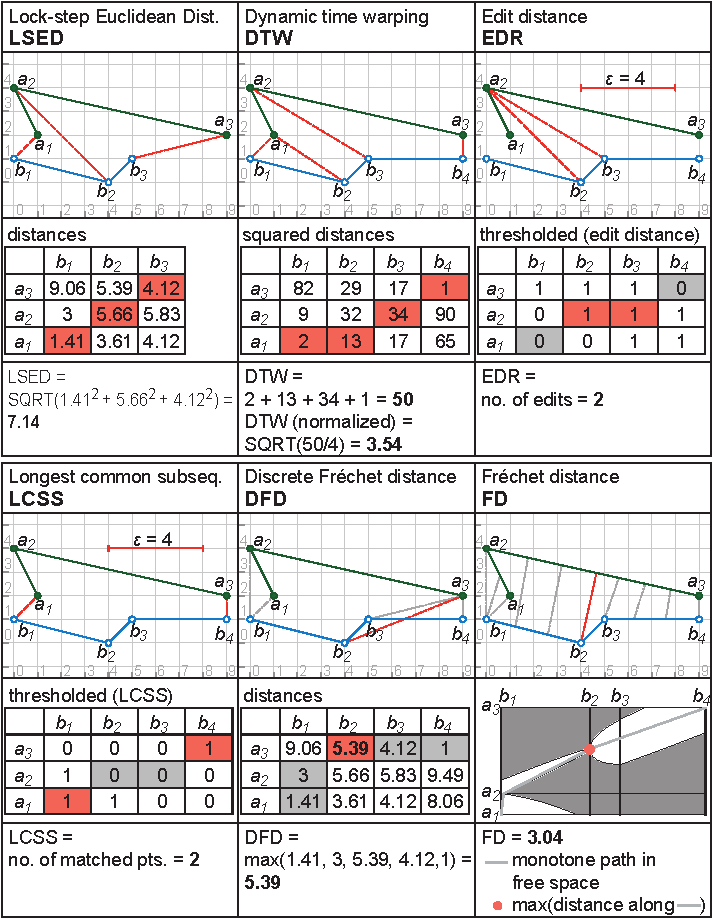
\includegraphics[width=110mm]{figures/Fig2}
\caption{Aligning two trajectories where n=3 and m=4 (except for LSED, where n=m=3) according to the various measures, along with a corresponding distance matrix or free-space diagram highlighting in red how each measure value is computed.}\label{fig:Traj_align}
\end{figure}

\subsection{Lock-step Euclidean distance (LSED)}

% Tests on Lock-step Euclidean distance will not be delivered here because of its .

%, with Lock-step Euclidean distance being the only measure mentioned that can reflect such similarity, for instance, by summing (in the discrete setting) or integrating (in the continuous setting) over time, or by taking the maximum distance over all times. 

If  $n=m$ we can interpret the trajectories as points in the Euclidean space $\mathbb{R}^{2n}$ and take their Euclidean distance.

\begin{definition}
The lock-step Euclidean distance distance of $A$ and $B$ is defined as
\[
Eu(A,B) = \sqrt {\sum_{i=1}^n \dist_2^2(a_i,b_i)}\;.
\]
\end{definition}

A frequently used variant is the average distance between corresponding measurements: 
\[
Eu'(A,B) = \frac{1}{n}\sum_{i=1}^n \dist_2(a_i,b_i)\;.
\]
Alternatively, the maximum instead of the average distance can be used.

If $s_i = t_i$ for all $1 \leq i \leq n=m$ then these distances measure how far the trajectories are apart at corresponding times. In particular, $Eu'(A,B)$ is then the average distance at corresponding times.
If we assume uniform sampling in time, then the requirement $n=m$ corresponds to both trajectories having the same duration, i.e., $s_n - s_1 = t_n - t_1$. However, if both trajectories have the same duration but use different sampling---possibly non-uniform, then we can generalize these measures using interpolation:
\[
Eu(A,B) = \frac{1}{n}\int_0^{s_n-s_1} \dist_2(A(t-s_1),B(t-t_1)) dt\;,
\]
 where $A(t)$ and $B(t)$ are the locations of A and B, respectively, obtained by interpolation. Most commonly linear interpolation is used for this, i.e., for $s_i \leq t \leq s_{i+1}$ we have

\begin{equation}
\label{eq:interpolated_traj}
 A(t) = a_{i+1} \frac{s_{i+1}-t}{s_{i+1}-s_i}  + a_i \frac{t -s_i}{s_{i+1}-s_i}\;.
\end{equation}

This interpolation assumes that the  object moves between two measurements with constant speed along a straight line; an alternative is to bound these distances only assuming an upper bound on the speed of movement~\cite{DBLP:conf/gis/BuchinP13}. All the distances above are easily computed in $O(n+m)$ time by scanning over the data once.

The Euclidean distance between two trajectories and its variants is widely used, see for instance~\cite{VlachosGK02}. A key assumption underlying these measures is that the two trajectories should be aligned using a strict correspondence in time.

All of the following measures relax this condition: data points with different time stamps may be aligned as long as the alignment preserves the order of the points along the trajectories. For all of the measures the alignment is optimized according to certain criteria. The measures differ in the specific criteria.


\subsection{Dynamic time warping (DTW)}
Dynamic time warping is a classical dynamic-programming algorithm, originally used for speech recognition, which has been successfully applied to time series data since the work by Berndt and Clifford~\cite{BerndtC94}.
Later, it became one of the most common methods for measuring similarity between trajectories.
The following definition follows the one presented by Chen et al.~\cite{ChenOO05}.

\begin{definition}
The dynamic time warping distance of A and B is is defined as
\[
DTW(A,B) =
\left\{
	\begin{array}{ll}
		0  & \mbox{if A and B are empty} \\
		\infty  & \mbox{if A or B are empty (not both)} \\
		\dist_2^2(a_1,b_1) +
		\min( \\
	DTW(A_{[2,n]},B_{[2,m]}), \\
			  DTW(A,B_{[2,m]}),  \\
			DTW(A_{[2,n]},B)) & \mbox{otherwise } \\
		\end{array}
\right.
\]
\end{definition}

\paragraph{Matrix formulation}
For this algorithm and several of the following ones, it will be insightful to interpret the distance definitions in terms of paths in the distance matrix between the trajectory points, illustrated in Fig.~\ref{fig:Traj_align} for two sample trajectories $A$ and $B$.
In the figure, the rows and columns of the matrix are laid out such that the squared distance between the first two points is at the lower left and the last two points at the upper right corner of the matrix.

%\begin{figure}[ht]
%\centering
%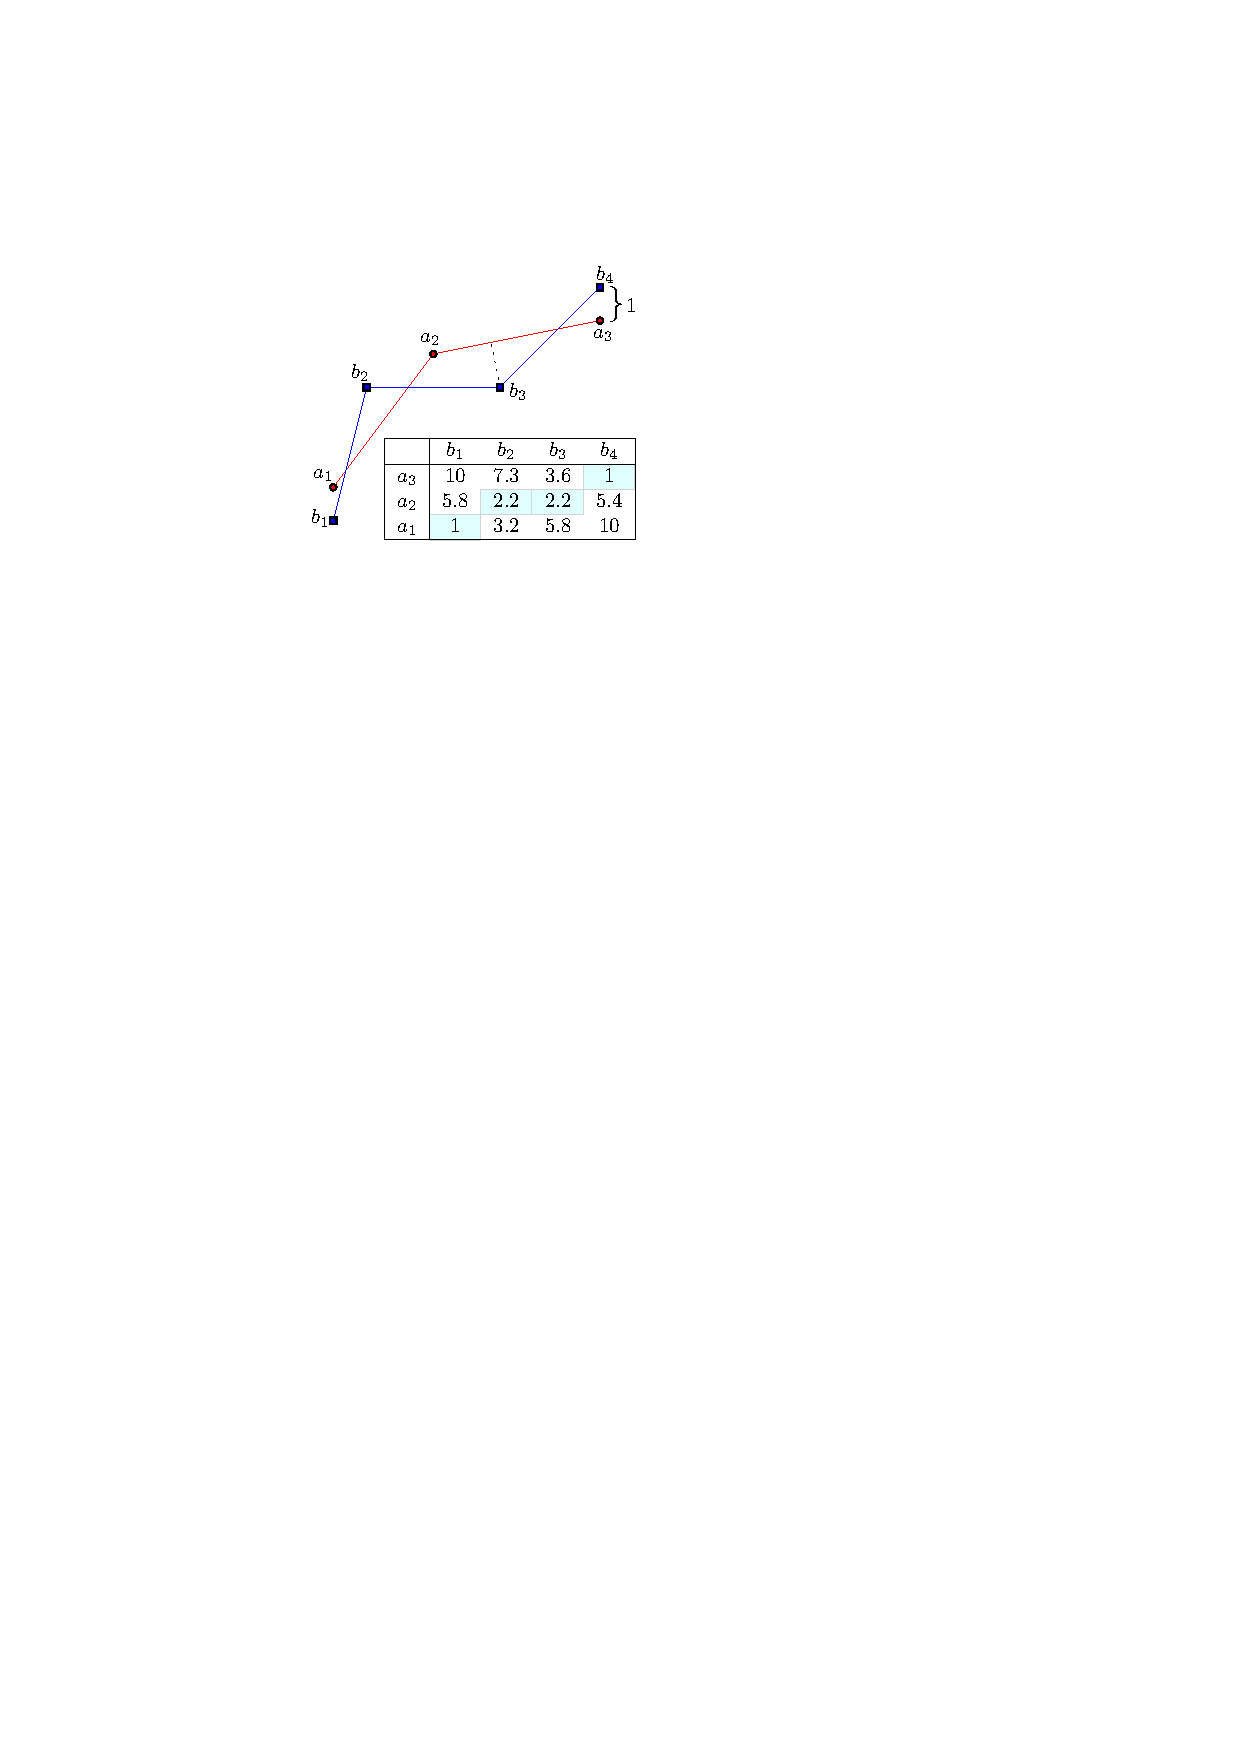
\includegraphics{figures/Fig1}
%\caption{Two trajectories and their distance matrix. In the distance matrix the optimal alignment according to DTW is highlighted.}\label{fig:DTW_eg} \end{figure}

Dynamic time warping can be seen as selecting a minimum cost path in the distance matrix.
More precisely, DTW selects a path from the lower left to the upper right corner of the distance matrix that minimizes the sum of squared distances. In the example, the resulting sum is $2 + 13 + 34 + 1
 = 50$. DTW is based on defining a cost for aligning two data points, namely the squared Euclidean distance between them.

From the point of view of walking along this path, from the lower left to the upper right corner, at each step DTW considers three possible moves: horizontal, vertical or diagonal.  More specifically, the options available are:
\begin{enumerate}
\item \textit{Match current pair of points, and move diagonally}: The cost of this move is equal to the squared distance between the pair of points.
\item \textit{Match current pair of points, and move up}: The cost is equal to the squared distance between the pair of points.
\item \textit{Match current pair of points, and move right}: The cost is equal to the squared distance between the pair of points.
\end{enumerate}

Another useful way to visualize the DTW approach is in terms of alignments. Each path in the distance matrix considered by DTW corresponds to an alignment between the points of the two trajectories (red dashed lines, Fig.~\ref{fig:Traj_align}). A path that goes through cell $(i,j)$, for $1 \leq i \leq n$ and $1 \leq j \leq m$, is implicitly aligning $a_i$ with $b_j$. 



What characterizes a similarity measure like DTW is how the cost of a path is defined, since the cost of a path represents how well the two trajectories are aligned in that path.  Following~\cite{ChenOO05}, we define the measure with squared Euclidean distances above. However, DTW is also frequently used with other costs, e.g., turning angles, discussed in more detail at the end of this section.

Therefore we can say that, in terms of alignments, DTW defines the cost of a path as the sum of the squared distances (or a different cost) between all pairs of aligned points. It is also common to enforce additional constraints on the path, for instance enforcing similar time-stamps between aligned measurements (see for example~\cite{keogh2005exact}).

\paragraph{Normalization}
The DTW distance corresponds to a sum of squared distances between data points and depends on the number of data points used. This makes it difficult to compare DTW distances between different numbers of data points in each trajectory. In the experiments we therefore divide the DTW distance by $\max (m,n)$, which is (in the matrix formulation) the smallest number of cells that need to be visited. To obtain a more intuitive measure, we additionally take the square root, that is, as normalized DTW distance we use $\sqrt{\frac{DTW(A, B)}{\max (m,n)}}$, which produces $\sqrt{\frac{50}{4}}=3.54$ for the example in Fig.~\ref{fig:Traj_align}.

It might seem natural to normalize using the number of values in the sum (in terms of the matrix formulation: the number of cells visited) instead of $\max (m,n)$. This approach would however make the normalized distance dependent on the path in the matrix, assigning relatively smaller normalized distances to longer paths. 

\paragraph{Algorithm}
The dynamic time warping distance is computed using dynamic programming, meaning that in terms of the formulation above one can compute for every cell $(i,j)$ the cost of the best path to reach it. This computation requires constant time per cell, as a cell's cost can be computed based on the cost of the cell left, below, and diagonally (left-below), resulting in an overall quadratic, i.e., $O(nm)$, computation time.
In practice, this can often be reduced to linear time, by carefully avoiding the computation for cells that have no influence on the final result~\cite{keogh2005exact}.


\subsection{Edit distance (EDR)}
Another common choice for comparing trajectories are measures based on edit distances.
Originally proposed to measure how similar two strings of characters are, edit distances have been successfully used for trajectory similarity.
In this section we present the variant proposed by Chen et al.~\cite{ChenOO05}, known as \emph{edit distance on real sequence (EDR)}.

\begin{definition}
The edit distance on real sequence (EDR) of $A$ and $B$ is is defined as
\[
EDR(A,B) =
\left\{
	\begin{array}{ll}
		n  & \mbox{if B is empty} \\
		m  & \mbox{if A is empty} \\
		\min( \\EDR(A_{[2,n]},B_{[2,m]})+\mbox{penalty}(a_1,b_1), \\
			  EDR(A,B_{[2,m]}) +1, \\
			EDR(A_{[2,n]},B)+ 1) & \mbox{otherwise } \\
		\end{array}
\right.
\]

where $\mbox{penalty}(a_1,b_1)$ is 0 if $\dist_\infty(a_1,b_1) < \epsilon $, or 1 otherwise.
\end{definition}
The definition uses a parameter $\epsilon$ as a matching threshold distance (i.e., two points closer than $\epsilon$ are considered to match).
\paragraph{Matrix formulation}
Similar to DTW, EDR searches for a minimum cost path in the distance matrix, although it uses a matrix where the cost is defined differently. As in DTW, there are three possible ways to move in the path towards the upper right corner:

\begin{enumerate}
\item \textit{Match current pair of points, and move diagonally}: The cost of this move depends on whether the current pair of points are considered to match (i.e., their distance is smaller than $\epsilon$).
In the former case there is no cost, in the latter the cost is one unit.
\item  \textit{Move right}: This costs one unit.
\item  \textit{Move up}: The cost is one unit.
\end{enumerate}

It is important to note that in EDR costs are thresholded to 0 if the current pair of points match, whereas in all other situations the cost is 1, irrespective of the distance between the current pair of points. This results in the \emph{distance threshold matrix}, a Boolean matrix as shown in Fig.~\ref{fig:Traj_align}.
However, non-thresholded versions also exist.
For instance, EDR itself is an adaptation of a measure proposed by Cai and Ng~\cite{NgC04}, called \emph{edit distance with real penalty} (ERP), where instead of penalizing with 1 every time two elements do not match, ERP penalizes with the squared distance between the non-matching elements.

%[\texttt{Caption of Fig. 3}: boolean matrix for thresholded distances for trajectories from Fig.~1.]
%\begin{figure}[ht]
%\centering
%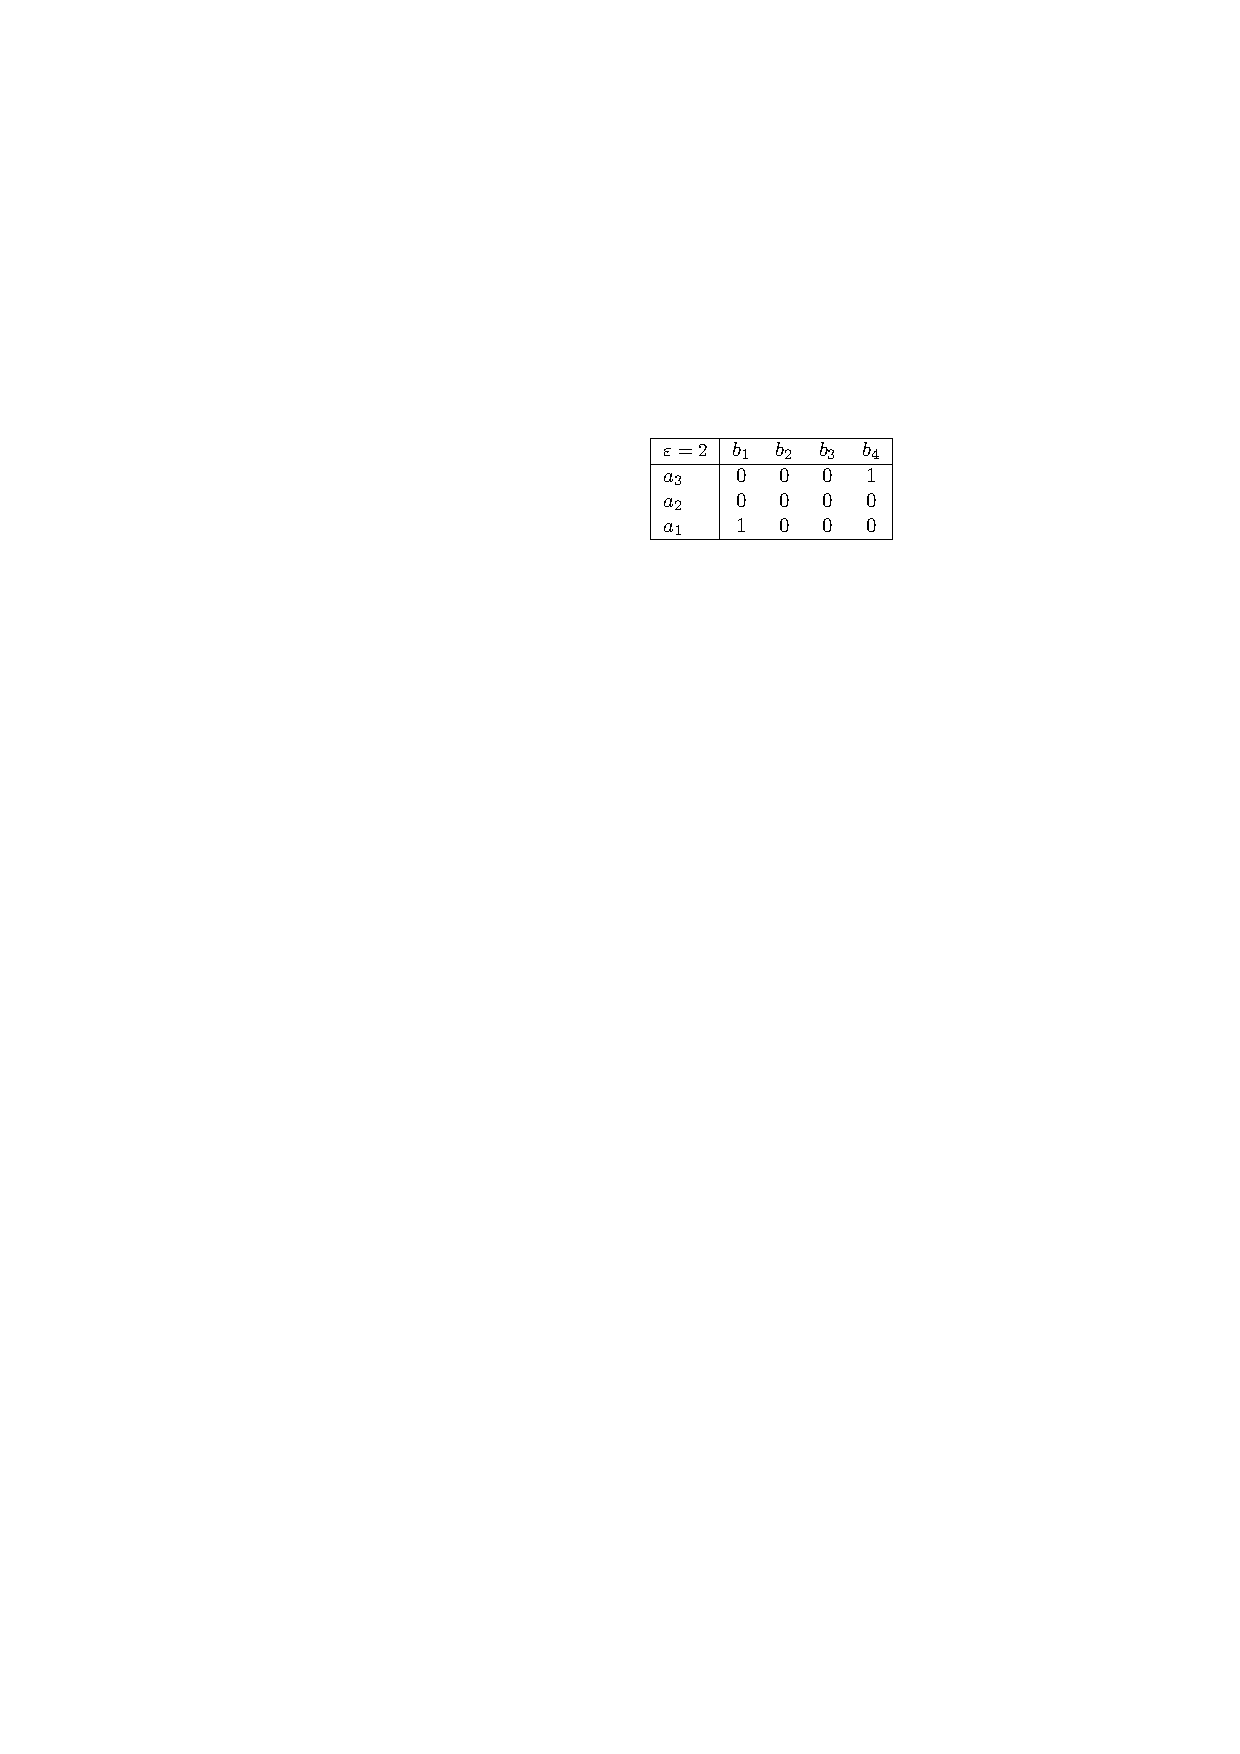
\includegraphics{figures/Fig3}
%\caption{Boolean matrix for thresholded distances for trajectories from Fig.~1.}\label{fig:Bool_matrix}
%\end{figure}

In terms of alignments, EDR defines the cost of a path as the number of aligned points that are not considered a match.

\paragraph{Algorithm}
Computing edit distances can be implemented in the same way as DTW and therefore take quadratic time (i.e., $O(nm)$) in the worst case.


\subsection{Longest common subsequence (LCSS)}
Measures based on longest common subsequences try to capture how well two trajectories match by measuring the length of the longest subtrajectory in common.
LCSS measures are closely related to edit distances, and have also received attention in the context of trajectory similarity.
The following definition follows Vlachos et al.~\cite{VlachosGK02}.

\begin{definition}
The length of the longest common subsequence between $A$ and $B$ is defined as
\[
LCSS(A,B) =
\left\{
	\begin{array}{ll}
		0  & \mbox{if A or B is empty} \\
		1+LCSS(A_{[1,n-1]},B_{[1,m-1]}) & \mbox{if } \dist_\infty(a_n,b_m) < \epsilon  \mbox{ and } \\ &|n-m| \leq \delta \\
		\max( LCSS(A_{[1,n-1]},B), \\ LCSS(A,B_{[1,m-1]})) & \mbox{otherwise } \\
		\end{array}
\right.
\]
\end{definition}

The definition uses two parameters, $\delta$ and $\epsilon$.
As in EDR, $\epsilon$ is a matching threshold distance (i.e., two points closer than $\epsilon$ are considered to match).
Additionally, $\delta$ controls how far in time (specifically, in timesteps) two matching points can be, in order to align the trajectories in time.
However, it should be noted that $\delta$ is not specific to LCSS, and could be added to any of the other measures.

\paragraph{Matrix formulation}
LCSS also looks for a path in its distance matrix (Fig.~\ref{fig:Traj_align}), although with a few differences with respect to the previous measures.
Firstly, the path is searched in the opposite direction: from the upper right to the lower left corner.\footnote{It is easy to modify the formula to go in the same direction as DTW and EDR, but we preferred to present the original formulation from~\cite{VlachosGK02}.}
Secondly, the goal is to find a path of \emph{maximum} cost, as the objective is to maximize the number of matched points.

As before, there are three possible ways to advance:
\begin{enumerate}
\item \textit{Match current pair of points, and move diagonally}: To be considered a match, the pair of points cannot be further than $\delta$ timesteps away. This movement gains (costs) one unit
\item \textit{Move left}: This movement results in no gain (cost).
\item \textit{Move down}: This movement results in no gain (cost).
\end{enumerate}

Similar to EDR, LCSS is thresholded, meaning that what is relevant is whether the point pairs match or not, but not their actual distances.
In terms of alignments, LCSS defines the value of a path as the number of alignments considered a match, making LCSS a measure that is somewhat complementary to EDR.

\paragraph{Algorithm}
As before, LCSS can be implemented using dynamic programming, and therefore takes quadratic time (i.e., $O(nm)$) in the worst case.

% Commenting out part about how to make it a distance
\iffalse
Now we can define a similarity function based on LCSS.

\begin{definition}
LCSS-based similarity measure and distance definitions for two trajectories $A$ and $B$.
\[
S(A,B)=\frac{LCSS(A,B)}{\min(n,m)}
\]
\[
D(A,B)=1-S(A,B)
\]
\end{definition}

Vlachos et al.~\cite{VlachosGK02} also give a second similarity measure that is invariant to translations, but here we only present the simplest version.
\fi


\subsection{Discrete Fréchet distance (DFD)}
Proposed by  Eiter and Mannila~\cite{Wien94computingdiscrete}, DFD can be seen as a version of DTW that takes the \emph{maximum} distance between aligned points along the path. This is in contrast to DTW, which considers the \emph{sum} of all squared distances.

\begin{definition}
The discrete Fr\'echet distance of $A$ and $B$ is defined as
\[
DFD(A,B) =
\left\{
	\begin{array}{ll}
		0  & \mbox{if A and B are empty} \\
		\infty  & \mbox{if A or B are empty (not both)} \\
		\max( \dist_2(a_1,b_1),
		\min( \\
	DFD(A_{[2,n]},B_{[2,m]}), \\
			  DFD(A,B_{[2,m]}),  \\
			DFD(A_{[2,n]},B)) & \mbox{otherwise } \\
		\end{array}
\right.
\]
\end{definition}

\paragraph{Matrix formulation}
Similar to DTW and EDR, DFD searches for a minimum cost path in the distance matrix, from the lower left to the upper right corner (Fig.~\ref{fig:Traj_align}). As in DTW, the cost of a pair is measured by taking the Euclidean distance, and there are three possible ways to advance:

\begin{enumerate}
\item \textit{Match current pair of points, and move diagonally}: The cost is equal to the distance between the pair of points, only if it is greater than or equal to the cost of the rest of the path.
\item \textit{Match current pair of points, and move up}: The cost is equal to the distance between the pair of points, only if it is greater than or equal to the cost of the rest of the path.
\item \textit{Match current pair of points, and move right}: The cost is equal to the distance between the pair of points, only if it is greater than or equal to the cost of the rest of the path.
\end{enumerate}

In terms of alignments, DFD defines the cost of a path as the maximum over the distances between all pairs of aligned points. Note that taking the squared distance instead of the distance would result in the same optimal paths. Essentially, DFD's difference from DTW is that it takes the maximum instead of the sum of the distances between all pairs of aligned points.

\paragraph{Algorithm} As before, DFD can be implemented using dynamic programming, resulting in an $O(nm)$-time algorithm.


\subsection{Fr\'echet distance (FD)}
All the distance measures above are discrete, in the sense that they only align the measured locations $a_i$, $b_i$. This can potentially lead to problems for non-uniform sampling.
In contrast, the Fr\'echet distance~\cite{ag-cfd-95} is \emph{continuous}, meaning that it considers alignments between all points in both trajectories, by using the interpolated trajectories $A(s), B(t)$ (defined as in Formula~\ref{eq:interpolated_traj}).

\begin{definition}
The Fr\'echet distance between $A$ and $B$ is defined as
\[
F(A,B) = \inf_{\sigma} \max_{t \in [s_1,s_n]} \dist_2(A(t),B(\sigma (t))),
\]

where the infimum is taken over all continuous, strictly monotone-increasing functions $\sigma \colon [s_1,s_n] \rightarrow [t_1, t_m]$ (i.e., all continuous alignments).
\end{definition}

This can be interpreted as the continuous version of the discrete Fr\'echet distance. Similarly, continuous versions of the other measures discussed above have been proposed.

\paragraph{Algorithm} Most algorithms to compute the Fr\'echet distance solve the decision problem as a subroutine. The decision problem for the Fr\'echet distance is to decide whether the Fr\'echet distance is smaller than a given $\epsilon > 0$. Given an algorithm for the decision problem, the actual distance can be approximated using for instance a binary search over $\epsilon$. A more complex search procedure, such as parametric search, can be used to compute the Fr\'echet distance exactly~\cite{ag-cfd-95}.

The decision problem can be solved by a simple dynamic programming algorithm. Consider the so-called \emph{free-space diagram} in Fig.~\ref{fig:Traj_align}, which is the continuous analog to the distance threshold matrix that is used for the edit distance and longest common subsequence problem. In this diagram the vertical axis corresponds to the parameter space of $A$ and the horizontal axis to the parameter space of $B$. Thus, the point $(s,t)$ in the diagram corresponds to the pair of points $(A(s), B(t))$. The free-space diagram for a given $\epsilon > 0$ is the set of points $(s,t)$ with the property that the distance between $A(s)$ and $B(t)$ is at most $\epsilon$.

In the figure, the free-space diagram for $\epsilon \approx 3.04$ is the white-colored region, and the monotone path in free-space is grey. The Fr\'echet distance is at most $\epsilon$ if and only if there is a path from the lower-left corner to the upper-right corner that goes through the free-space and is monotonically increasing in both coordinates. To compute whether such a path exists we can incrementally compute the part of the free-space diagram that is reachable by such a path. This results in an $O(mn)$-time algorithm for the decision problem. Computing the exact Fr\'echet distance then requires an additional $\log (mn)$ factor for the parametric search~\cite{ag-cfd-95}. In the example of Fig.~\ref{fig:Traj_align} the exact Fr\'echet distance is approximately 3.04 as the white region would disconnect when $\epsilon$ is decreased further. The corresponding alignment is illustrated as a dashed red line.

\subsection{Lessons from the conceptual and theoretical analysis}
Following our pen-and-paper conceptual and theoretical analysis, this section summarizes the main aspects in which the measures differ.

% Metric: Yes to: LSED, DFD, FD, perhaps ED (\emph{edit distance with real penalty}~\cite{NgC04}), but not EDR; No to DTW, LCSS, EDR
% Continuous: Yes to FD; maybe LCSS (partial Fr\'echet distance~\cite{bbw-09}); maybe summed or average Fr\'echet distance~\cite{b-cfdts-07} and ~\cite{efrat2007curve}, continuous version of DTW; no LSED, DFD, ED. 
% Absolute time: LSED; all others relative time. 
% Absolute space: No for all with transformations; A no for all except LSED and FD using transformation invariant properties
% Computational differences 
% This is done by first making an analysis of the ways in which the measures differ before discussing the decision process involved in selecting one particular measure over the others.

% Recall that most of the measures discussed align two trajectories and in this way take time into account qualitatively.


\subsubsection{Metric versus non-metric}

When a similarity measure is used for clustering and indexing, it is desirable that the chosen measure is metric. Among the measures discussed, LSED, DFD, and FD are metrics, whereas the others are not because: 
\begin{itemize}
\item DTW does not obey the triangle inequality;
\item LCSS does not measure difference (instead measuring, to some extent, similarity), although variants that satisfy some weaker conditions can be defined~\cite{VlachosGK02}; and
\item EDR does not fulfill two of the conditions, namely the identity of indiscernibles ($D(A, B) = 0$  if and only if   $A = B$)  and the triangle inequality ($D(A, B) + D(B, C) \geq D(A, C)$) are not preserved by EDR.
\end{itemize}
However, it should be noted that edit distance in general may be a metric, including some variants of edit distance used for time-series analysis, such as \emph{edit distance with real penalty}~\cite{NgC04}.

\subsubsection{Discrete versus continuous}

As the name suggests, Fr\'echet distance (FD) is the continuous version of discrete Fr\'echet distance (DFD). It is this continuity that makes FD distinct from the other similarity measures considered here. The goal for FD is to find a continuous alignment; that is, one between the complete path of both trajectories, as opposed to an alignment between only the trajectory points. While implementing a continuous measure does present additional computational challenges, as opposed to the relative simplicity of a discrete measure, the worst-case running time of the FD is only slightly worse than of the other measures.

While we only discuss the FD as continuous version of the DFD, continuous versions of some other measures have also been defined. The so-called ``partial Fr\'echet distance''~\cite{bbw-09} is the continuous analogue of LCSS. For a given $\epsilon >0$, the partial Fr\'echet distance aligns two trajectories to maximize the parts that have distance at most $\epsilon$, measuring the overall length of these parts. The summed or average Fr\'echet distance is a continuous version of dynamic time warping, and aligns the trajectories as to minimize the average distance between matched points~\cite{b-cfdts-07}. Continuous versions of dynamic time warping using other measures for the pairwise distance between matched points have also been considered~\cite{efrat2007curve}.

\subsubsection{Relative versus absolute time}
LSED is a similarity measure that only compares measurements at corresponding times. As such, LSED takes a very different approach from the other measures discussed, which aim at temporally aligning the two trajectories. 

Common to all of the other discussed similarity measures, DTW, ED, LCSS, DFD, and FD, is the guiding principle of temporally aligning the two trajectories by aggregating the local costs (i.e., the cost of the temporal alignment between each pair of points). The key differences between measures often lie in the details of how this is done. For instance, DTW and DFD fundamentally differ only on whether to take the sum (DTW) or the maximum (DFD) of the local costs.

\subsubsection{Relative versus absolute space}

The distance measures as considered above align trajectories in time to minimize absolute Euclidean distances. However, depending on the application, relative distance may be more relevant. For instance, one might want to consider a trajectory and a shifted copy of it as essentially the same. This is addressed in two different ways.

The first approach is to take one of the measures above and optimize it under a suitable set of transformations, e.g., translations. That is, if $D(A,B)$ is a distance measure between trajectories $A$ and $B$, one would consider $\min \{d(A,B + \tau)\;|\; \tau \in T \}$, where $T$ is the set of two-dimensional translations. This minimization problem is typically computationally expensive (see for example~\cite{VlachosGK02}), and often solved by sampling the space of transformations~\cite{as-sm-12}.

The second approach is much simpler: instead of using Euclidean distances, an alternative measure that is invariant under a suitable set of transformations is used. Common choices for this measure include heading (translation-invariant) and turning angle (translation- and rotation-invariant), any of which can be applied to the similarity measures discussed above. For instance, one can use DTW with turning angles instead of squared Euclidean distances. To that end, the turning angle must be defined for each point $a_i$. This is usually done by considering points $a_{i-1}$ and $a_{i+1}$, and computing the angle between vectors $\overrightarrow{a_{i-1} a_{i}}$ and $\overrightarrow{a_{i}a_{i+1}}$. Note that the use of measures such as heading or turning angle complicates the application of continuous similarity measures such as FD, since it would require to interpolate heading or turning angle between trajectory points. This is, in general, hard to do in a meaningful way; for instance, turning angle is always zero between points if linear interpolation is used.

\subsubsection{Computational efficiency}

Regarding efficiency, the simplest and fastest measure discussed is LSED, as it only requires processing the input trajectories once, which takes $O(n+m)$ time.
All the dynamic programming-based measures, namely DTW, EDR, LCSS and DFD, require $O(nm)$ time, at least in their standard formulations.
An advantage of the dynamic programming approach is that it is easy to implement, and it is almost identical for all four measures.
Theoretical improvements for some of these measures are possible, see for example \cite{DBLP:conf/icde/2002,bbmm-fswd-14,Masek198018}.
However, these are minor improvements on theoretical running times that come at the cost of an increase in the complexity of the implementation.
In practice, it is possible to get better running times. For instance for DTW there is an algorithm that typically runs in linear time~\cite{keogh2005exact}. FD is the least efficient similarity measure, requiring $O(mn\log mn)$ time. 

\subsubsection{Outliers}

One final difference between the various measures worth highlighting is the way in which they deal with outliers. Generally, measures that use the maximum distance between matched points (such as FD and DFD) emphasize large distances and are therefore more sensitive to outliers than measures that use the sum of distances (or the sum of squared distances). Thresholds (as used in the EDR and LCSS) can be useful for dealing with outliers as they allow for the assignment of a uniform cost to pairs that are matched but have a distance larger than the threshold. In this sense, LCSS can be interpreted as the measure that minimizes the number of points that need to be classified as outliers to perfectly align the remaining trajectories. This, however, comes at the cost of introducing the threshold as an additional parameter.

\subsection{A key to choosing a suitable similarity measure}

Summarizing our discussion of the  theoretical and conceptual differences between each of the similarity measures is investigated above, Table \ref{tab:key}  captures the salient differences between the measures.  The table provides a visual guide as to whether each similarity measure is a metric; operates on continuous trajectories; temporally aligns trajectories; can be used following spatial transformation of trajectories (relative space following transformation); can be used with a distance measure that is invariant under transformation (relative space using invariant distance);  compares the relative computational efficiency;  and compares the measure robustness to outliers. Note that for the last two categories more stars indicate better performance. 

\begin{table}[htb]
    \caption{Summary of differences in similarity measures}\label{tab:key}
\renewcommand{\arraystretch}{2}
    \begin{tabular}{>{\raggedright\arraybackslash}p{2.8cm}|>{\raggedright\arraybackslash}p{1.25cm}>{\raggedright\arraybackslash}p{1.25cm}>{\raggedright\arraybackslash}p{1.25cm}>{\raggedright\arraybackslash}p{1.25cm}>{\raggedright\arraybackslash}p{1.25cm}p{1.25cm}}
~                                        & LSED     & DTW         & EDR         & LCSS        & DFD      & FD      \\ \hline
    Metric?                                  & Yes      & \cellcolor{gray!30}  No          & \cellcolor{gray!15} No, but see \cite{NgC04}& \cellcolor{gray!30} No          & Yes      & Yes     \\
    Continuous?                              & \cellcolor{gray!30} No       & \cellcolor{gray!15} No, but see \cite{b-cfdts-07} & \cellcolor{gray!30} No          & \cellcolor{gray!15} No, but see \cite{bbw-09} & \cellcolor{gray!30} No       & Yes     \\
    Relative time?                           & \cellcolor{gray!30} No       & Yes         & Yes         & Yes         & Yes      & Yes     \\
    Relative space following transformation? & Yes      & Yes         & Yes         & Yes         & Yes      & Yes     \\
    Relative space using invariant distance? & \cellcolor{gray!30} No       & Yes         & Yes         & Yes         & Yes      & \cellcolor{gray!30} No      \\
    Computational efficiency?                & $\star\star\star$  & \cellcolor{gray!15} $\star\,\star$    & \cellcolor{gray!15} $\star\,\star$    & \cellcolor{gray!15}$\star\,\star$    & \cellcolor{gray!15}$\star\,\star$ & \cellcolor{gray!30}$\star$ \\
    Outliers?                                & \cellcolor{gray!15}$\star\,\star$ & \cellcolor{gray!15}$\star\,\star$    & $\star\star\star$        & $\star\star\star$        & \cellcolor{gray!30} $\star$     & \cellcolor{gray!30} $\star$    \\
    \end{tabular}
\end{table}
% You may title this section "Methods" or "Models".
% "Models" is not a valid title for PLoS ONE authors. However, PLoS ONE
% authors may use "Analysis"
	
\section{Experiments}
As highlighted in Section~\ref{sub:conceptual}, our aim is not to identify a single similarity measure that fits all situations; rather  our aim is to clarify  the differences and similarities between measures. The decision on which similarity measure to apply depends on each individual definition of distance, with different applications placing  the emphasis  on different aspects of the trajectories they compare. 

Having already explored these differences from a conceptual and theoretical standpoint, in this section we aim to explore these through real data, enabling us to distinguish between differences which may be theoretically important, but practically less relevant.


\subsection{Datasets}
\label{sub:datasets}

To clarify the differences between measures, we calculated similarities for trajectories with contrasting properties: vehicle movements through a transportation network, and trajectories capturing the behavior of coastal wading birds. 
	
Our first dataset used is the Dublin bus GPS sample data~\cite{DublinBus}.  This dataset was selected to support experiments exploring the impacts spatial or temporal factors have on similarity measures independently. This dataset is suitable for separating spatial and temporal impacts because the trajectories can be fixed in one dimension and varied in the other. For example, a group of bus trajectories from the same bus route taken at different periods of a day can be identical in their spatial path, but have quite different temporal features. A representative subsample of bus trajectories were extracted from four weekdays (2nd, 3rd, 4th, and 7th of January 2013) and 8--9am, 1--2pm, and 8--9pm time blocks. This selection mechanism allows trajectories to be grouped based on temporal similarity as well as spatial similarity. Trajectory segments at the start or the end of a trajectory, where the bus was considered to be stationary, were removed as such a high level of similarity would likely dominate any similarity measures used. Two example pairs of trajectories are shown in Fig~\ref{fig:eg_bus}. 

\begin{figure}[ht]
	 \centering
	 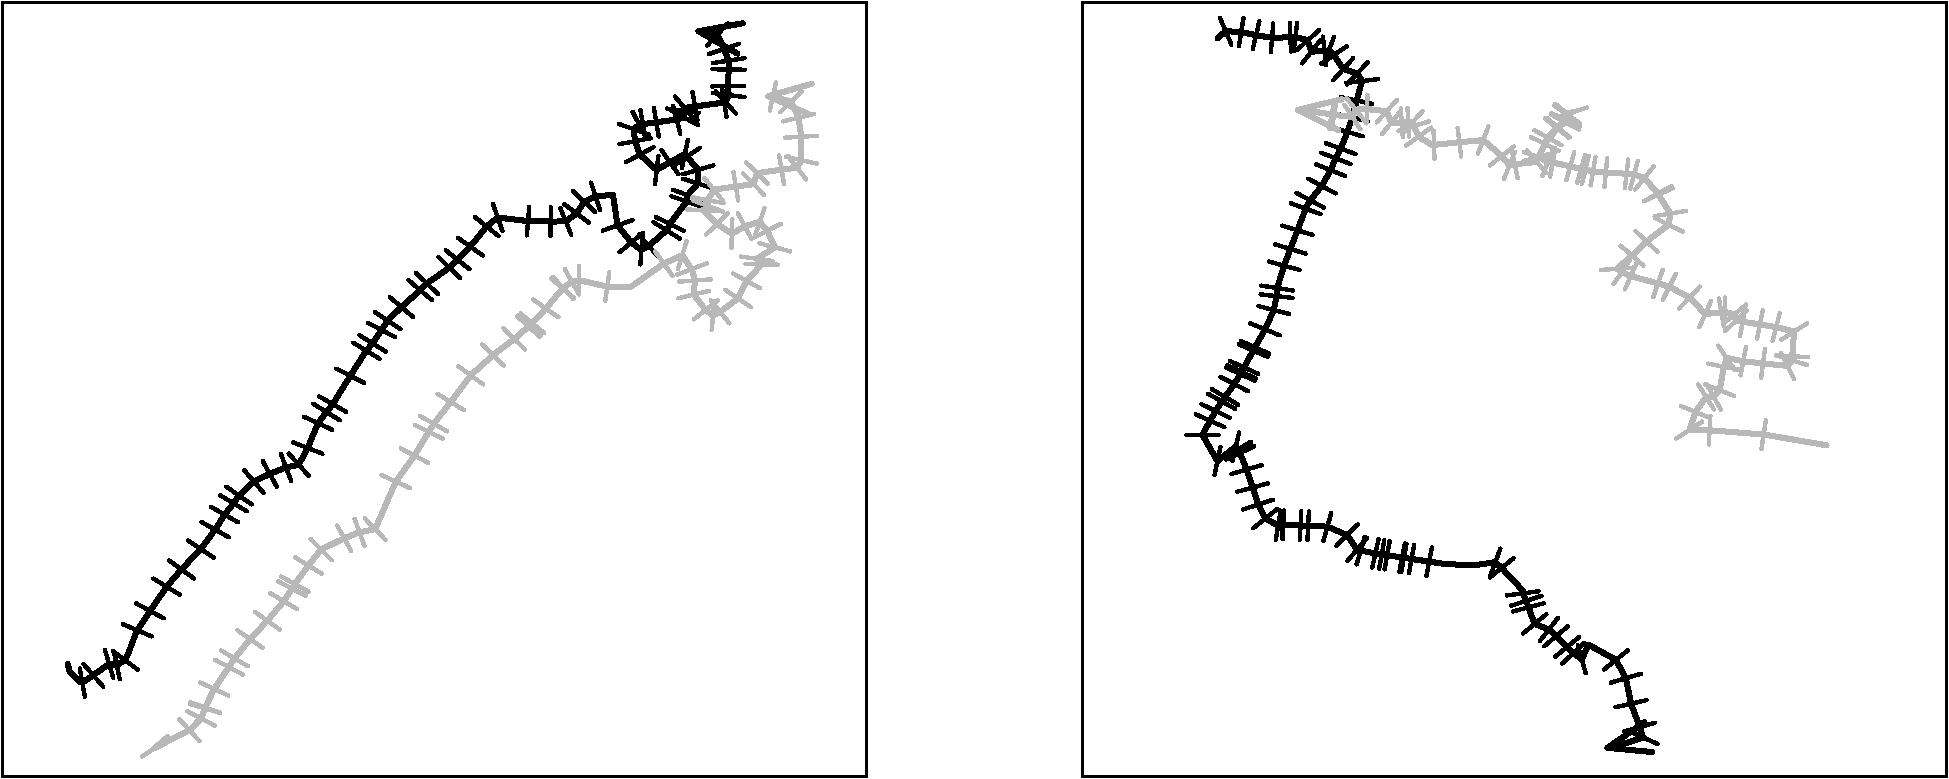
\includegraphics[width=120mm]{figures/busRoutesComparison}
	 \caption{Example bus trajectories. The left pair shows trajectories of the same bus route collected at the same time but on different days; the right pair shows trajectories with different routes and different times. Grey trajectories have been displaced for clarity.}
	 \label{fig:eg_bus}
\end{figure} 

The second dataset used is GPS data on oystercatchers tagged with bird activities~\cite{shamoun2012sensor}. This dataset was selected to provide comparison cases between trajectories with known behavioral differences. Specifically, trajectories governed by the activities of flight and forging were extracted for analysis. A minimum trajectory length of three fixes was set to exclude trajectories that are too short to clearly indicate any embedded activity.  
This dataset is suitable for tests on similarity measures where transformation in time and space is required, as trajectories reflecting the same activity may occur in different locations, direction, and speeds. It is the features that are invariant under certain spatial or temporal transformations that make such trajectories distinguishable, and therefore represent the different underlying activities. For example, one such feature for oystercatcher trajectories is that birds are more likely to make sudden turns when they are foraging compared to cases when they are simply flying (Fig.~\ref{fig:illu_flight_forage}).

\begin{figure}[ht]
	\centering
	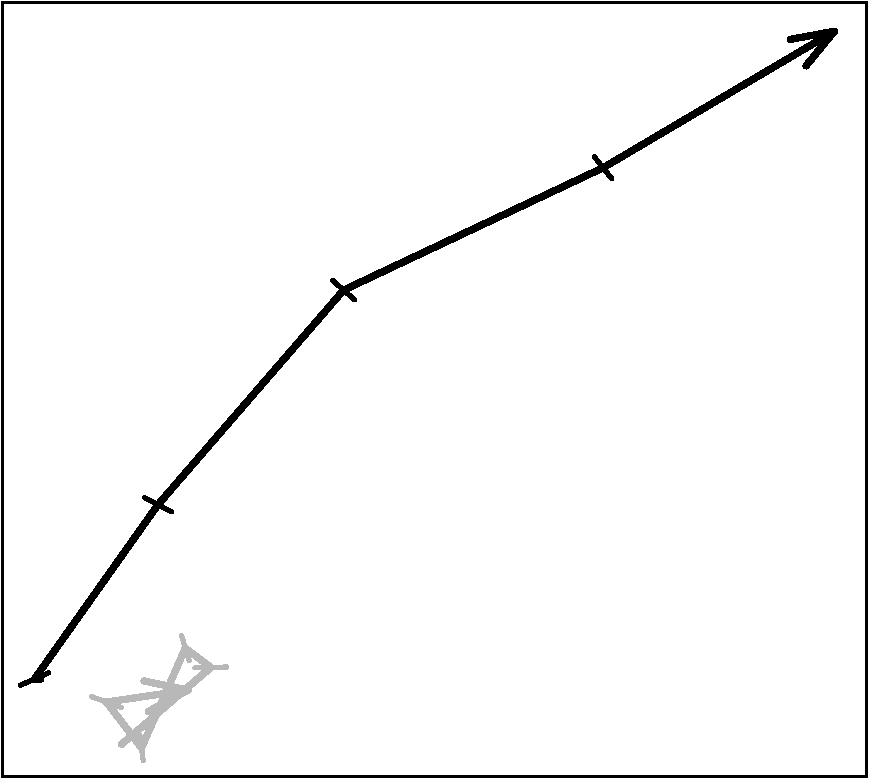
\includegraphics[width=60mm]{figures/birdComparison}
	\caption{One trajectory of flight (black) and one trajectory of foraging (gray)}
	\label{fig:illu_flight_forage}
\end{figure}


\subsection{Experiment 1}
\label{par:experiment_1}
Our first experiment examined the similarity measures when applied to a single high resolution trajectory under different transformations (Fig.~\ref{fig:sample bus}). A base trajectory was created by regular sub-sampling from the raw data (Fig.~\ref{fig:sample bus}a). Obviously, we expect all trajectory measures to find maximum similarity when trajectories are identical, and such a comparison can be seen as a trivial verification of the implementation of our code.  We then calculated similarity under the following conditions: 

\begin{enumerate}
\item A temporal transformation, where points were sub-sampled from the original trajectory with an increasing temporal interval, clustering points towards the (temporal) beginning of the trajectory (Fig.~\ref{fig:sample bus}b);
\item A spatial transformation where the base trajectory was rotated slightly about its origin (Fig.~\ref{fig:sample bus}c); and
\item A spatiotemporal transformation where both temporal and spatial transformations  above were applied (Fig.~\ref{fig:sample bus}d).
\end{enumerate}

\begin{figure}[ht]
	 \centering
	 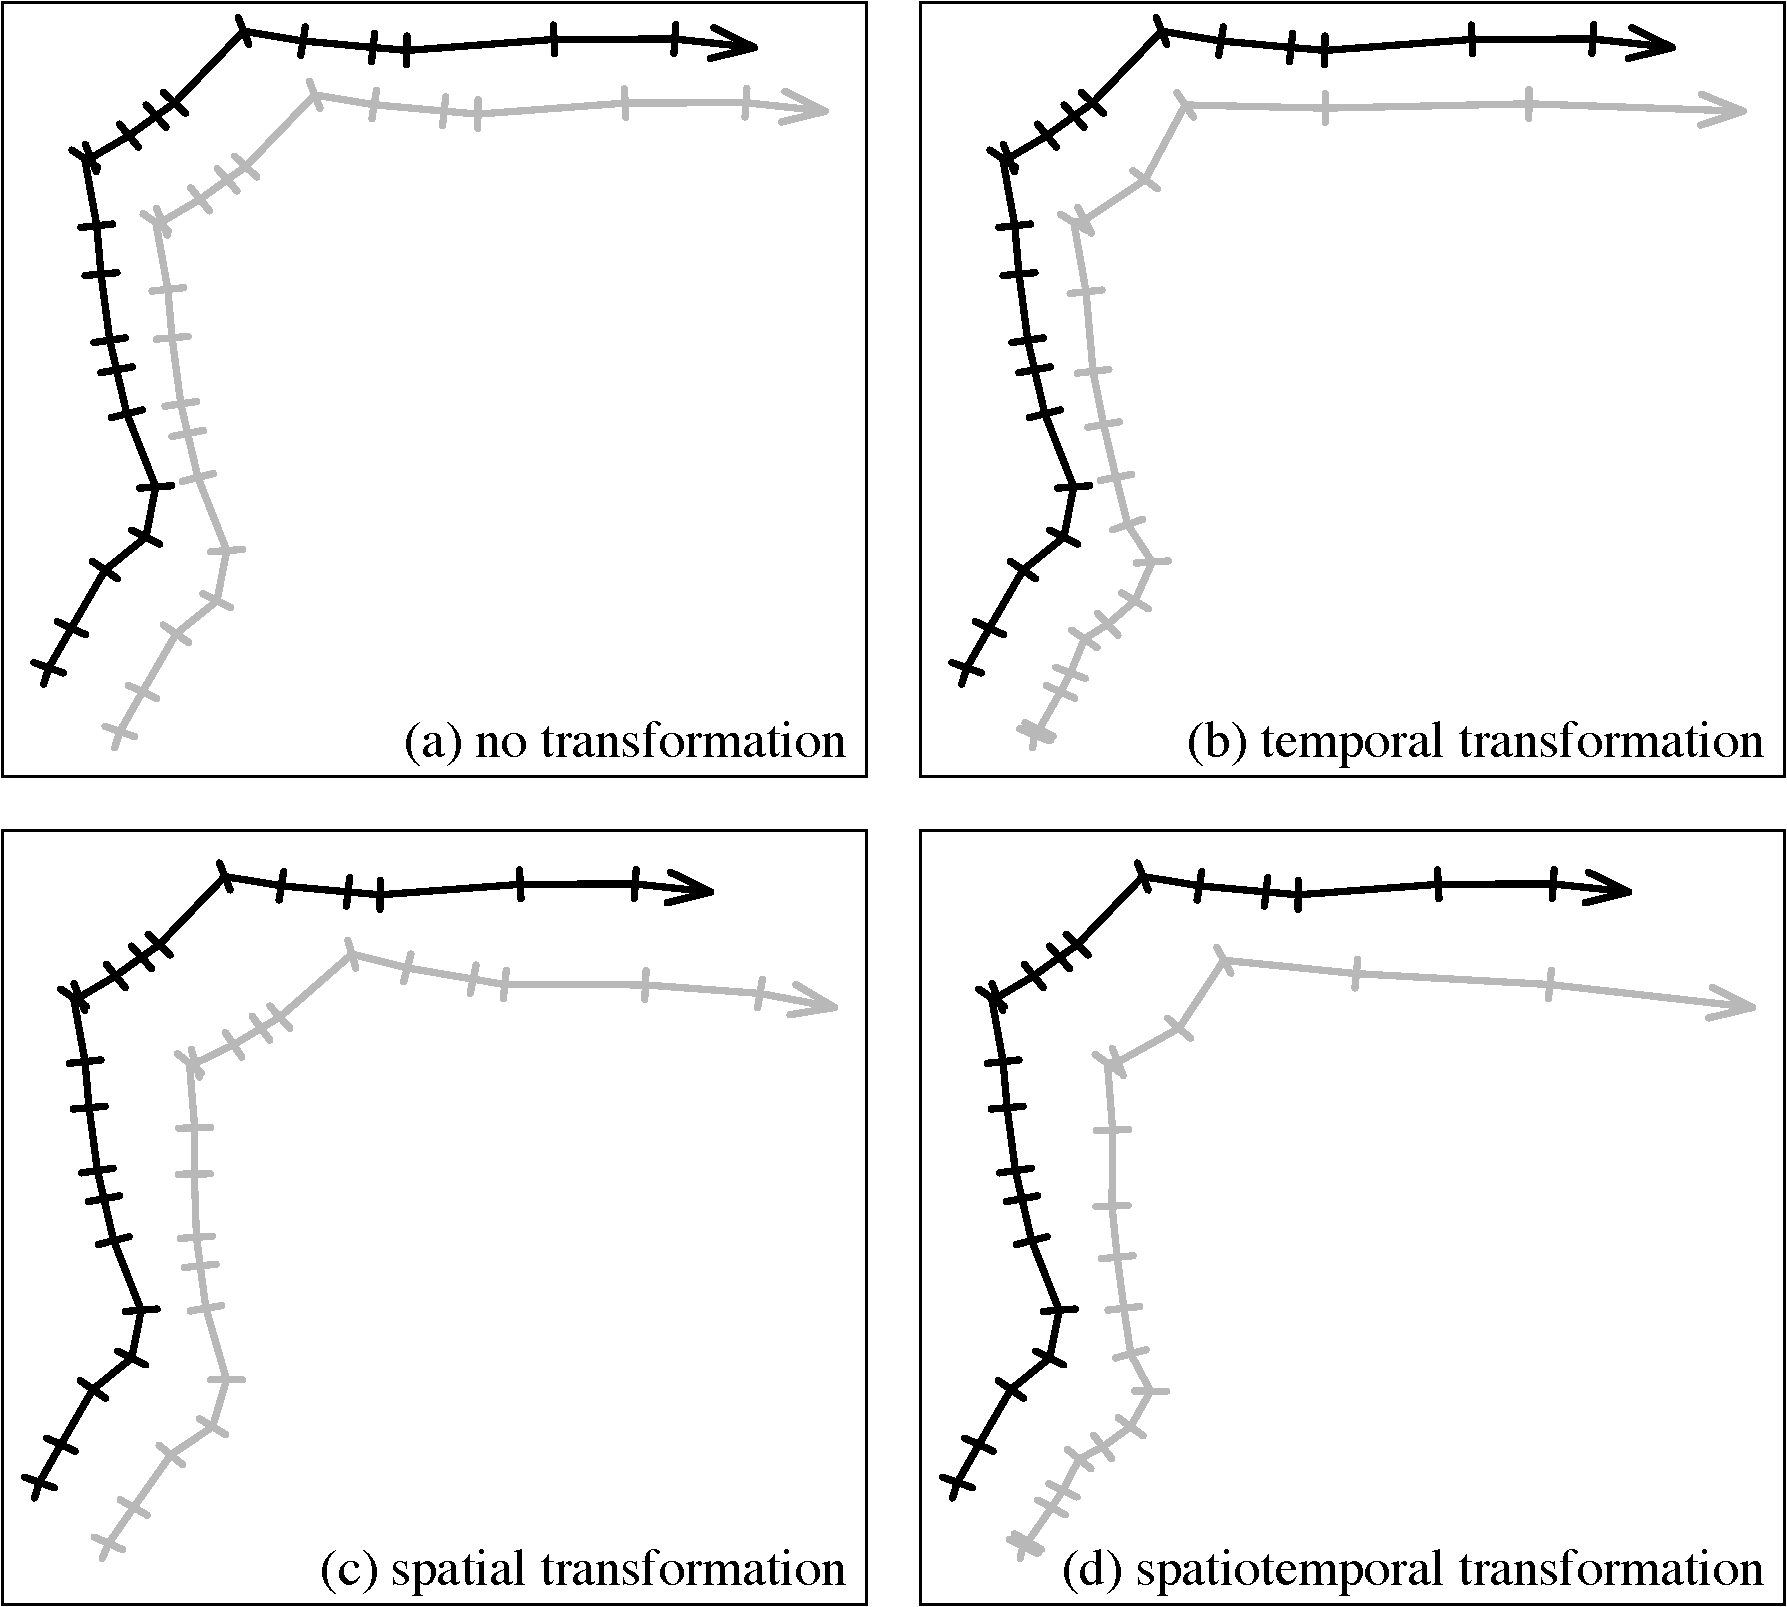
\includegraphics[width=110mm]{figures/trajectoryComparisons}
\caption{Trajectory comparisons between one bus trajectory and its variations}
%(a) no transformation, (b) temporal transformation, i.e., measurements are temporally shifted towards one the begin of the trajectory, (c) spatial transformation, i.e., the gray trajectory has been rotated, and (d) spatiotemporal transformation, i.e., the combination of both the spatial and the temporal transformation.}	
\label{fig:sample bus}	
\end{figure}

In this experiment we are interested in the ordering of results within and between similarity measures. In other words, are the same trajectory pairs always more similar, irrespective of the similarity measure used, or, as we expect from our theoretical analysis, are some measures more sensitive to spatial or temporal transformations than others?


\subsection{Experiment 2}
\label{par:experiment_2}
In our second experiment, we aimed to explore the behavior of different similarity measures on real trajectories constrained in a network space. Here, we assumed that spatial behavior, while not identical, is very similar for repeated instances of the same route, whereas temporal behavior may vary greatly (i.e., from variations in traffic flow). A key question then is: which similarity measures are better suited to discriminating between trajectories paired from different categories? We chose two dimensions along which to characterize trajectories: spatial similarity, where we select trajectories according to individual bus routes; and temporal similarity, where we select trajectories from the three sampled time periods (8--9am, 1--2pm, and 8--9pm, all on weekdays). These criteria were then used to randomly select 36 pairs of trajectories to test four scenarios:
\begin{itemize}
\itemsep-1ex
\item \emph{SameSame}: Pairs of trajectories along the same route in the same temporal window.
\item \emph{SameRoute}: Pairs of trajectories along the same route in different temporal windows.
\item \emph{SameTime}: Pairs of trajectories along different routes in the same temporal window.
\item \emph{DiffDiff}: Pairs of trajectories along different routes in different temporal windows.
\end{itemize}

These four scenarios capture the essential spatial and temporal dimensions of empirical trajectory similarity in network space. We hypothesize that similarity measures will be able to discriminate between trajectories along these dimensions.  

\subsection{Experiment 3} % (fold)
\label{par:experiment_3}
In Experiment 3 we compared empirical trajectories of oystercatcher data. Here our aim was to assess trajectory similarity with respect to existing behavioral labels (flight and foraging). We hypothesized that similarity measures should be able to discriminate between such behaviors. In this experiment, pairs of trajectories were selected randomly from labeled foraging behavior and from all of the small number of available flight trajectories to build the following comparison sets:

\begin{itemize}
\itemsep-1ex
\item \emph{FlyFly}: Pairs of trajectories labeled as flight.
\item \emph{FlyForage}: Pairs of trajectories labeled as flight and foraging.
\item \emph{ForageForage}: Pairs of trajectories labeled as foraging.
\end{itemize}

These comparisons are a typical example of trajectory similarity comparisons in a between-subjects experiment in ecology, where the aim is to describe animal behaviors using GPS tracks. Since such behavioral patterns need not take place within the same space, and we are interested in the general properties of the trajectories, a necessary first step is a spatial transformation (translation and rotation) to align trajectories. All trajectories were translated such that their origins were identical, and rotated so that the angle formed between the first and last point in every trajectory was 45 degrees. We hypothesized that similarity measures would capture differences between behavioral patterns through spatial behavior.


\subsection{Experiment 4}
\label{par:experiment_4}
In any experiments comparing methods, it is important to consider straightforward baselines that are easy to interpret. Since the two datasets used exhibit very different properties, another experiment with transformation in space allowed was designed to compare two more general activities---bird activity and bus activity.
As the bird and bus trajectories lie far away from each other, transformation in space and time was utilized to enable comparison. 
The similarity measures were then performed on three types of trajectory pairs:

\begin{itemize}
\itemsep-1ex
\item \emph{BirdBird}: Pairs of bird trajectories.
\item \emph{BusBird}: Pairs of bird and bus trajectories.
\item \emph{BusBus}: Pairs of bus trajectories.
\end{itemize}

Based on this pairing schema, a random set of both bird and bus trajectories were used to examine whether bus and bird are distinguishable based solely on their movement patterns.


\subsection{Measure normalization}\label{sec:measurenormalization}
As the trajectories used in the experiments can vary dramatically in length, a direct comparison of similarity measures is not possible. In order for all similarity measures to be compared within the same categories, and between inter-category groups, LCSS, DTW, and EDR similarity values needed to first be normalized. LCSS was normalized by the shortest trajectory length while DTW and EDR were normalized by the longest trajectory length.  As DFD and FD are essentially unaffected by length of trajectories, normalization was unnecessary.
Additionally, the threshold value $\epsilon$ for LCSS and EDR was set to 100m for the first experiment while 50m was chosen for the later experiments. 


\section{Results and interpretation}
\label{sec:results}

\subsection{Experiment 1}
\label{par:result_1}
In our first experiment we sought to explore the difference between similarity measures under a range of transformations. As introduced above, our expectation is that some similarity measures are more sensitive to spatial or temporal transformations than others. Fig.~\ref{fig:sample bus} shows the trajectories compared, while Table~\ref{tab:Exp1} shows the values calculated for each similarity measure. 

\begin{table}[ht]
\centering
\caption{Computed similarities between black and gray trajectories in Fig.~\ref{fig:sample bus}. The ranks in parentheses indicate for every measure the relative order of the computed similarities.}\label{tab:Exp1}

\begin{tabular}{l|rrrr}
Transformation& None & Temporal & Spatial & Spatiotemporal \\
 & (Fig.~\ref{fig:sample bus}a) & (Fig.~\ref{fig:sample bus}b) & (Fig.~\ref{fig:sample bus}c) & (Fig.~\ref{fig:sample bus}d) \\ \hline
LCSS Ratio & $1~(1)$ & $0.68~(2)$ & $0.61~(3)$ & $0.55~(4)$ \\ 
\rowcolor{gray!15} EDR Ratio & $0~(1)$ & $0.57~(3)$ & $0.43~(2)$ & $0.70~(4)$\\ 
Fréchet (m) & $0~(1)$ & $163.61~(2)$ & $497.84~(3)$ & $497.84~(3)$ \\ 
\rowcolor{gray!15} Discrete Fréchet (m) & $0~(1)$ & $456.87~(2)$ & $497.84~(3)$ & $497.84~(3)$ \\ 
DTW (m) & $0~(1)$ & $179.64~(2)$ & $270.19~(4)$ & $259.10~(3)$ \\
\end{tabular}
\end{table}

It is important to note that a physical interpretation of the meaning of the similarity measures in all cases except FD and DFD, which can be directly interpreted as a discrete physical distance, distance is difficult. EDR and LCSS are both normalized between 0--1, while DTW is normalized as a function of the number of points in the longest trajectory in a pair (see Section~\ref{sec:measurenormalization}). 

A number of observations can be made from Table~\ref{tab:Exp1}. Firstly, our implementations of the similarity measures deliver expected values for identical trajectories, a trivial but important sanity check. 

Secondly, similarity values are indeed sensitive to the measures used, with variation in the ranking of trajectory similarity between measures as a function of transformations.

Thirdly, in this experiment a clear difference is visible in the distances associated with continuous and discrete Fréchet distance under temporal transformations. This difference arises since under FD distances are calculated between not only data points, but also interpolated segments between these points, and thus the influence of the temporal transformation of the data points is limited. 


    

\subsection{Experiment 2}
\label{par:result_2}
In our second experiment we explored the sensitivity of the similarity measures to comparisons between the trajectories of buses in Dublin for four spatiotemporal scenarios. Our hypothesis was that different similarity measures should be able to discriminate between trajectories that differ spatially and temporally.  

Fig.~\ref{fig:bus_all} shows box plots of the similarity measures for each case. The first observation that can be made is that spatial difference between trajectories dominates all similarity measures. This is visible in the clear differences across all measures between \emph{SameSame} and \emph{SameRoute} (which compare the same spatial trajectory paths) versus \emph{SameTime} and \emph{DiffDiff} (which compare different routes). By contrast, temporal differences appear to have little to no influence on the properties of the similarity measures. 

This observation was confirmed using a Wilcoxon signed rank hypothesis test. The test revealed no significant differences at the 5\% level between either the \textit{SameSame} versus \textit{SameRoute} or the \textit{SameTime} versus \textit{DiffDiff} across all measures tested. By contrast, the differences between \textit{SameSame} versus  \textit{SameTime}/\textit{DiffDiff} and between the \textit{SameRoute} versus  \textit{SameTime}/\textit{DiffDiff} are significant at the 5\% level in all cases. 

This result implies that differences between trajectories on a network, calculated using the measures we investigate, are largely the product of spatial differences. However, the fact that bus routes are oftentimes designed to be spatially different in order to cover more area and share less overlap may be a factor in the lack of similarity between different routes, when compared with different times. Further, bus trajectories collected at different time periods are not necessarily temporally distinct in the way illustrated by the temporal transformation of a trajectory in Experiment 1. Instead, there appeared to be limited difference in the proportion of points at each section of the trajectory. This is likely due to buses following fixed schedules, operating at similar speeds, and stopping with similar frequency.


    
\begin{figure}[ht]
	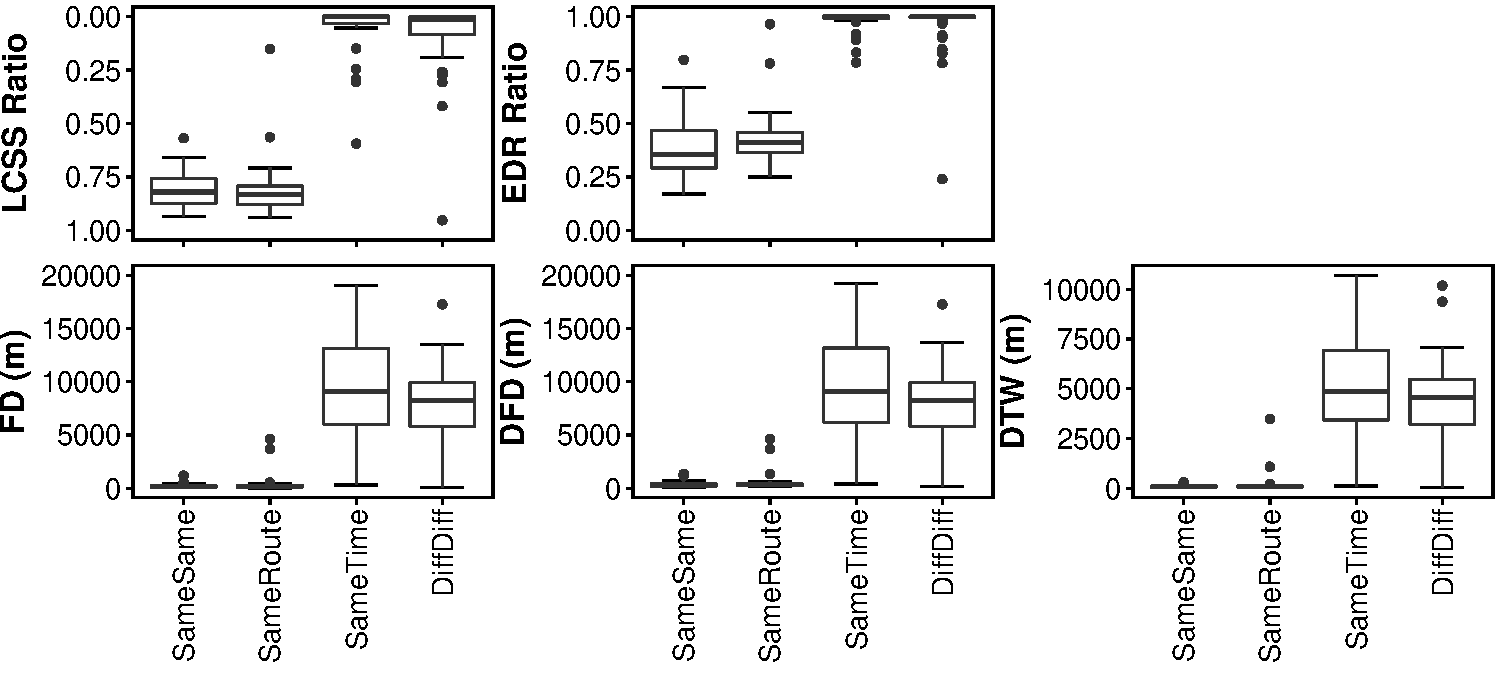
\includegraphics[width=\linewidth]{figures/Exp2}
	\caption{Box plots of bus trajectory similarity} \label{fig:bus_all}
\end{figure}

% \begin{table}[ht]
% 	\centering
% 	\caption{P-values for the Wilconxon signed rank tests on SameSame vs. SameRoute and DiffDiff vs. SameTime from Figure~\ref{fig:bus_all}).}
% 	\begin{tabular}{|c|c|c|}
% 		\hline
% 		& {\bf SameSame vs. SameRoute} & {\bf DiffDiff vs. SameTime} \\ \hline
% 		{\bf LCSS Ratio} & $0.4463$ & $0.1864$ \\ \hline
% 		{\bf EDR Ratio} & $0.0743$ & $0.7368$ \\ \hline
% 		{\bf Fréchet} & $0.6694$ & $0.1763$ \\ \hline
% 		{\bf Discrete Fréchet} & $0.2592$ & $0.1763$ \\ \hline
% 		{\bf DTW} & $0.4507 $ & $0.1115$ \\ \hline
% 	\end{tabular}
% 	\label{tab:bus_same_route}
% \end{table}

\subsection{Experiment 3}
\label{par:result_3}
In our next set of experiments, we explored the ability of similarity measures to discriminate between different activities with very clear spatiotemporal signatures (cf. Fig.~\ref{fig:illu_flight_forage}). Box plots showing the results for all five similarity measures are  shown in Fig.~\ref{fig:bird_activity}. It was expected that trajectories governed by the same activity would be more alike, whereas trajectories for different activities would show greater difference. 

\begin{figure}[ht]
	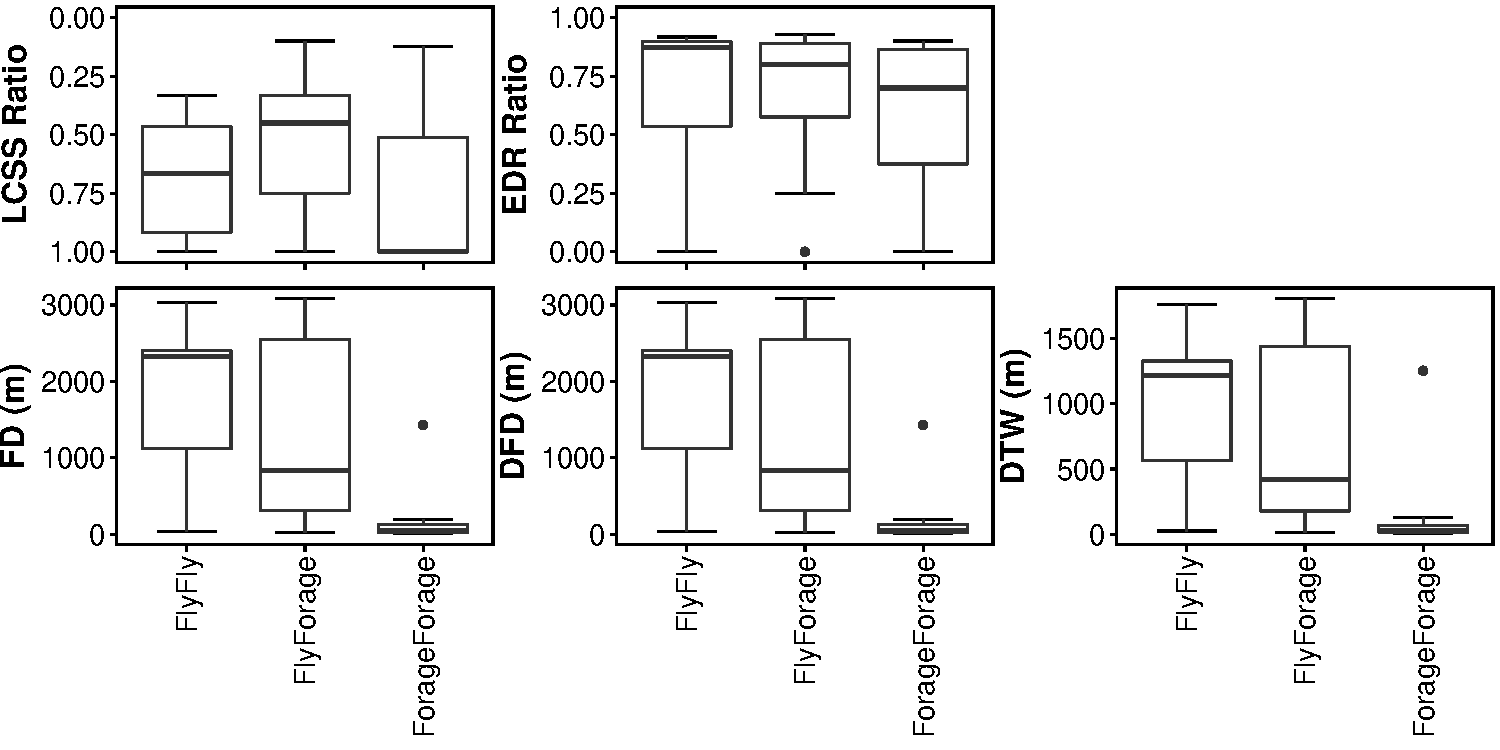
\includegraphics[width=\linewidth]{figures/Exp3}
	\caption{Box plots of bird activity trajectory similarity} \label{fig:bird_activity}
\end{figure}

In contrast to the previous experiment, the results do show a clear difference between the five similarity measures, with only Fréchet distance, DFD, and DTW showing obvious differences in similarity values. While pairs of foraging trajectories were ranked with higher similarity by Fréchet distance, DFD, and DTW, this was not the case for pairs of flight trajectories, exhibiting little difference from pairs of flying and foraging trajectories. These greater similarity values indicate that foraging trajectories share a large extent of common features that are invariant to transformation. Conversely, the weaker similarity values for the other two groups points to  the explanation that one flight trajectory may as dissimilar from other flight trajectories, as it is from foraging trajectories. For the EDR Ratio, there appears to be little or no difference between any of the sets of pairs, indicating that EDR is unable to distinguish the exhibited movement patterns. The LCSS ratio however does appear to exhibit the expected signal (i.e., that pairs of flying and pairs of foraging trajectories have greater similarity than mixed pairs), albeit one that is very weak.

To test whether similarity measures could be treated as being drawn from different populations, according to the semantics of the comparisons, we performed a Kruskal-Wallis rank sum test (Table~\ref{tab:kruskal_wallis}). As suggested by the box plots, we found significant differences (p$<$0.05) between the similarity values for Fréchet distance, DFD, and DTW. To further explore the nature of these differences, we then performed pairwise Wilcoxon signed rank tests to compare the (FlyFly with FlyForage/ForageForage with FlyForage) (Table~\ref{tab:wilcoxon_oyster}). We found significant differences (p$<$0.05) for both measures when comparing foraging behavior with mixed groups of trajectories, but were not able to distinguish between flying behavior from mixed groups. These results, given our previous experiment, imply that the form of trajectories has an influence on the sensitivity of measures to differences.

\begin{table}[ht]
	\centering
	\caption{P-values for Kruskal-Wallis test performed on the similarity distribution for analysis on Oystercatcher data.}
	\begin{tabular}{l|rl}
		& P-value& Significant at 5\% level\\ \hline
		LCSS Ratio & $0.3389$\  \\
		\rowcolor{gray!15} EDR Ratio & $0.5583$\ & \\
		Fréchet & $0.0057$ & * \\
		\rowcolor{gray!15} Discrete Fréchet & $0.0057$ & * \\
		DTW & $0.0075$ &* \\
	\end{tabular}
	\label{tab:kruskal_wallis}
\end{table}

\begin{table}[ht]
	\centering
	\caption{P-values for Wilcoxon signed rank tests for analysis on Oystercatcher data.}
	\begin{tabular}{l|lrl}
		& Comparison groups & P-value& Significant at 5\% level\\ \hline
		\multirow{2}{*}{FD, DFD} & {FlyVsFly and FlyVsForage} & $0.4375$ & \\ 
		&  {ForageVsForage and FlyVsForage} & $0.0210$ & *\\ \hline
		\multirow{2}{*}{DTW} & {FlyVsFly and FlyVsForage} & $0.5625$ & \\ 	
		& {ForageVsForage and FlyVsForage} & $0.0210$ & *\\ 	
	\end{tabular}
	\label{tab:wilcoxon_oyster}
\end{table}


\subsection{Experiment 4}
\label{par:result_4}
In our fourth experiment we compared trajectories from our two datasets, to explore the ability of similarity measures to cluster fundamentally different types of behavior (buses moving in a structured network space versus birds free to move in a potentially unconstrained space). This experiment provides a baseline for all experiments by comparing trajectories from very different domains that are expected to be intrinsically very different (bus movement and bird movement). 

Figure~\ref{fig:BusBird} shows box plots for trajectories selected from pairs of similar (\textit{BusBus} and \textit{BirdBird}) and dissimilar (\textit{BusBird}) trajectories. Here we note that Fréchet distance, DFD, and DTW all appear to be able to discriminate between semantically similar and dissimilar objects, with largest values (and thus most dissimilar) trajectories associated with the \textit{BusBird} pairs. However, LCSS and EDR, while finding the greatest similarity between \textit{BirdBird} pairs, found either higher dissimilarity (LCSS) or  comparably high dissimilarity (EDR) between \textit{BusBus} and \textit{BusBird} pairs. As for Experiment 3, pairwise Wilcoxon signed rank tests were performed in order to determine if there was a significant difference between the three groups of trajectory pairs. With the exception of the EDR ratio on \textit{BusBird} and \textit{BusBus} trajectory pairs, all other comparisons  deferred exhibit significant differences at the 5\% level.

\begin{figure}[h]
	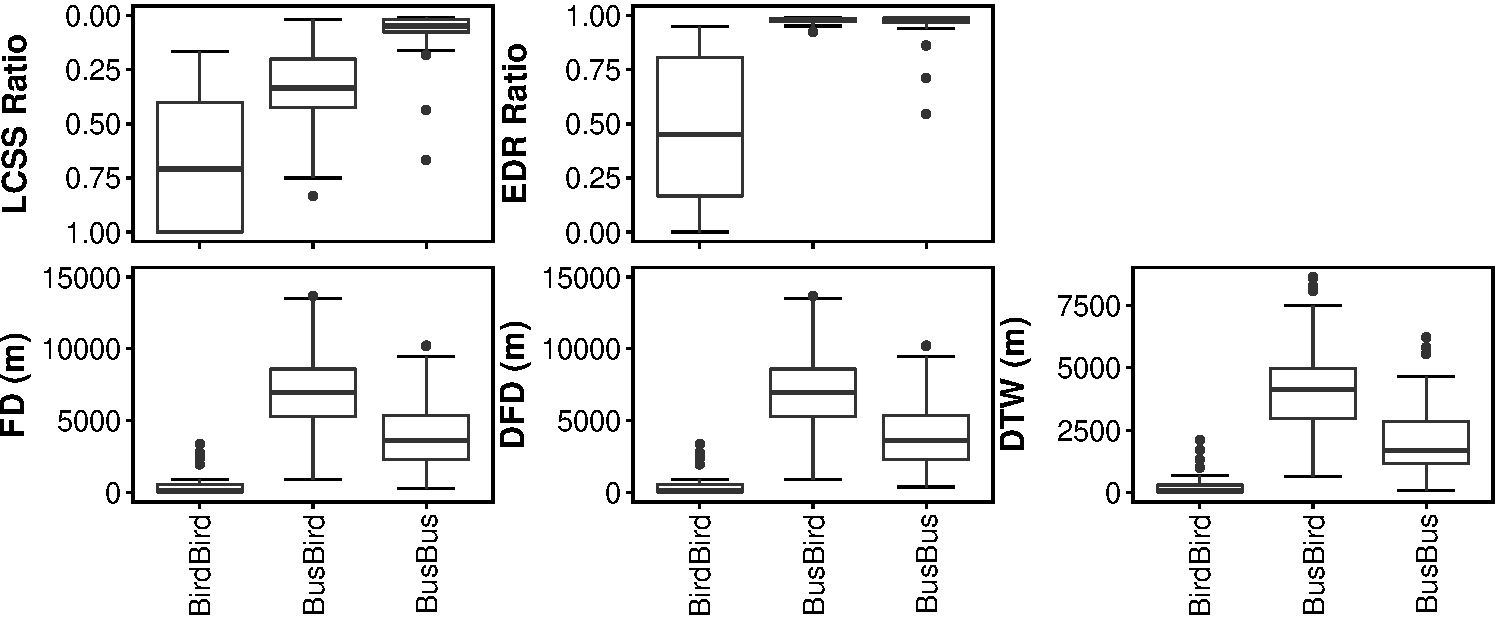
\includegraphics[width=\linewidth]{figures/Exp4}
	\caption{Box plots of bird and bus activity trajectory similarity} \label{fig:BusBird}
\end{figure}

\subsection{Summary of experimental results}

In summary, based on the differences observed across our four experiments, we infer three general and empirical properties of the different similarity measures.

\begin{enumerate}

\item Differences in similarity values are sensitive to the choice of measure. The relative ordering of similarity  for a fixed set of trajectories can be expected to differ under different similarity measures. 

\item All tested similarity measures are better at distinguishing spatially dissimilar trajectories, when compared with temporally dissimilar trajectories. Relatively small spatial differences in trajectories tend to correspond to large differences in the magnitude of  measured similarity than even  relatively large temporal differences in trajectories. 

\item Broadly speaking DTW, DFD, and FD tended to outperform LCSS and EDR in our experiments.  In Experiment 3, LCSS and EDR both failed to distinguish trajectories that arose from quite different activities, and were at least visually quite distinct (Fig.~\ref{fig:illu_flight_forage}). In Experiment 4, the similarity values for EDR even failed to enable discernment apart the dissimilarity between different bus trajectories when compared with the dissimilarity between bus and bird trajectories. 
\end{enumerate}
 	
\section{Conclusions and recommendations}
\label{sec:discussion}

We conclude with the following observations and recommendations on the use of different trajectory similarity measures. 

\paragraph{Metric measures}  Some applications, such as indexing or clustering, rely on similarity measures that offer metric properties. In such cases only some of these similarity measures are suitable (LSED, DFD, FD, and possibly edit distance, although not EDR). 
 	
\paragraph{Discrete vs continuous measures} The majority of the similarity measures evaluated were discrete (considering only the measured locations for each trajectory). Only Fréchet distance, and its interpolation between measured locations, can provide a measure of difference over continuous trajectory paths, although some continuous analogs of DTW and LCSS can also offer continuous measure properties. 

\paragraph{Computational efficiency} A major factor to consider when selecting a similarity measure is computational efficiency. In theory, FD is the least efficient measure; LSED the most efficient; with DTW, LCSS, EDR, DFD all underpinned by similar dynamic programming implementations. However, in practice throughout all of the experiments, little to no difference was found when comparing FD to its discrete counterpart. In all cases, the primary influence in execution time is the number of sample points in the trajectories, meaning that over-sampling should be avoided.

\paragraph{Maximum vs sum of distances} %(or: wide/narrow perspective, holistic/atomistic, instantaneous/global)
Similarity measures at root measure either the \textit{maximum} of distance between trajectories (i.e., FD, DFD), or the \textit{sum} of all or a sample of distances  between trajectories (LSED, DTW, EDR, LCSS). Different measures in this respect may lend themselves to different applications. As a direct consequence, those measures that are based on maximum distances are much more sensitive to outliers than those based on the sum of distances. That said, in our experiments FD, DFD, and DTW performed similarly, indicating that any outliers present in our datasets were not sufficiently significant to influence the results.
 	
\paragraph{Spatial vs temporal similarity}
In all of the similarity measures tested, the spatial differences between trajectories were more important in determining the magnitude of measured similarity than temporal differences. This is particularly evident in Experiment 2. However, the precise  magnitude of these differences is likely to depend strongly on the specific application.

\paragraph{Thresholds} This exploration has not  covered the selection of meaningful thresholds  for similarity  measures that require them, EDR and LCSS. Neither theory nor the experiments in this  paper can offer insights into the right thresholds to choose. Thresholds are highly data dependent,  and their selection needs to take into account the specific characteristics of the application, including noise, outliers, and constrained or unconstrained spaces for movement.  

\paragraph{Bounded versus unbounded measures}
As noted among the five similarity measures, LCSS and ED can be expressed as ratios, bounded between $0$ and $1$. Fréchet distance, DFD, and DTW are unbounded positive numbers. Though bounded measures do enable similarity results to be compared across different datasets, they have low resolution when representing high dissimilarity. For example, while it is easy to define 0 in edit distance ratio as two trajectories that are identical, there is no situation where two trajectories are so different that they produce a value of $1$. Additionally, this low resolution poses significant issues when different types of trajectories are compared as evidenced by LCSS and EDR ratio's inability to distinguish different movement patterns in Experiment 3.

% \paragraph{General versus specific patterns}
%Despite various levels of transformation, trajectories tend to be more diverse when they are clustered based on a more general pattern. For example, bus trajectories of the same route show a high degree of similarity with each other, whereas one bird trajectory in general can be quite different from another bird trajectory. Additionally, even for the same level of abstraction, some patterns are simply  harder to extract using the discussed similarity measures. The diversity of trajectories for flight activity as opposed to foraging activity shown by experiment 3 is a clear example of this. 


%	\section{Conclusion} % (fold)
%	\label{sec:Conclusion}
%	Triggered by the hardness of a decision, which one has to make in choosing a suitable similarity measure for more complicated trajectory mining tasks, six trajectory similarity measures were evaluated and compared in great detail in theoretical definitions. 
%	Four among them were then evaluated on trajectories with various levels of transformation being allowed. 
%	With hoping variation in transformation can represent the essences for most application scenarios, all four measures seem applicable for trajectory comparison allowing temporal transformation while Fréchet distance and DTW ratio show advantages in extracting similarity from activities when both spatial and temporal transformation are allowed. 
%	Admittedly, the type of transformation is highly subject to application scenarios and so is the choice for similarity measure.   


% Do NOT remove this, even if you are not including acknowledgments.
\section*{Acknowledgments}
This work was initiated as a result of a Lorentz Center Workshop, \textit{Geometric Algorithms in the Field}, 23--27 June 2014, at Leiden University, Netherlands. Prof Duckham and Dr Both receive research funding support from the Cooperative Research Centre for Spatial Information (CRCSI) under the Rapid Spatial Analytics Program.
R. Silveira is supported by projects MINECO MTM2015-63791-R, Gen.\ Cat.\ DGR2014SGR46, and by MINECO through the Ram{\'o}n y Cajal program. P. Laube thanks the Institute of Natural Resource Sciences at the Zurich University of Applied Sciences (ZHAW) for supporting his research. 


\nolinenumbers

% Either type in your references using
% \begin{thebibliography}{}
% \bibitem{}
% Text
% \end{thebibliography}
%
% or

\bibliography{trajectory_similarity}


\end{document}

